%%%%%%%%%%%%%%%%%%%%%%%%%%%%%%%%%%%%%%%%
% Classe do documento
%%%%%%%%%%%%%%%%%%%%%%%%%%%%%%%%%%%%%%%%
\documentclass[bacharelado]{unb-cic}

%%%%%%%%%%%%%%%%%%%%%%%%%%%%%%%%%%%%%%%%
% Pacotes importados
%%%%%%%%%%%%%%%%%%%%%%%%%%%%%%%%%%%%%%%%

\usepackage[american,brazil]{babel}
\usepackage[brazil]{translator}
\usepackage[utf8]{inputenc}
\usepackage[T1]{fontenc}
\usepackage{indentfirst}
\usepackage{natbib}
\usepackage{xcolor,graphicx,url,epstopdf}
\usepackage{epigraph}
\usepackage{amsmath,amssymb,amsthm}
\usepackage {pdfsync}
\usepackage{float}
\usepackage{subfig}
\usepackage{listings}
\usepackage{color}
\usepackage{amsmath}
\usepackage{lscape}
\usepackage{rotating}
\usepackage{textcomp}
\usepackage{comment} 
\usepackage{multirow}
\usepackage{booktabs}
\usepackage{hhline}
 

%\bibpunct[; ]{(}{)}{,}{a}{}{;}%muda colchetes para parênteses

%%%%%%%%%%%%%%%%%%%%%%%%%%%%%%%%%%%%%%%%
% Cores dos links
%%%%%%%%%%%%%%%%%%%%%%%%%%%%%%%%%%%%%%%%

% Veja o arquivos cores.tex se quiser ver que outras cores estão
% pré-definidas.  Utilizando o comando \hypersetup abaixo nós
% evitamos aquelas caixas vermelhas feias em volta dos links.

%%%%%%%%%%%%%%%%%%%%%%%%%%%%%%%%%%%%%%%%%
% Cores do estilo Tango
%%%%%%%%%%%%%%%%%%%%%%%%%%%%%%%%%%%%%%%%

\definecolor{LightButter}{rgb}{0.98,0.91,0.31}
\definecolor{LightOrange}{rgb}{0.98,0.68,0.24}
\definecolor{LightChocolate}{rgb}{0.91,0.72,0.43}
\definecolor{LightChameleon}{rgb}{0.54,0.88,0.20}
\definecolor{LightSkyBlue}{rgb}{0.45,0.62,0.81}
\definecolor{LightPlum}{rgb}{0.68,0.50,0.66}
\definecolor{LightScarletRed}{rgb}{0.93,0.16,0.16}
\definecolor{Butter}{rgb}{0.93,0.86,0.25}
\definecolor{Orange}{rgb}{0.96,0.47,0.00}
\definecolor{Chocolate}{rgb}{0.75,0.49,0.07}
\definecolor{Chameleon}{rgb}{0.45,0.82,0.09}
\definecolor{SkyBlue}{rgb}{0.20,0.39,0.64}
\definecolor{Plum}{rgb}{0.46,0.31,0.48}
\definecolor{ScarletRed}{rgb}{0.80,0.00,0.00}
\definecolor{DarkButter}{rgb}{0.77,0.62,0.00}
\definecolor{DarkOrange}{rgb}{0.80,0.36,0.00}
\definecolor{DarkChocolate}{rgb}{0.56,0.35,0.01}
\definecolor{DarkChameleon}{rgb}{0.30,0.60,0.02}
\definecolor{DarkSkyBlue}{rgb}{0.12,0.29,0.53}
\definecolor{DarkPlum}{rgb}{0.36,0.21,0.40}
\definecolor{DarkScarletRed}{rgb}{0.64,0.00,0.00}
\definecolor{Aluminium1}{rgb}{0.93,0.93,0.92}
\definecolor{Aluminium2}{rgb}{0.82,0.84,0.81}
\definecolor{Aluminium3}{rgb}{0.73,0.74,0.71}
\definecolor{Aluminium4}{rgb}{0.53,0.54,0.52}
\definecolor{Aluminium5}{rgb}{0.33,0.34,0.32}
\definecolor{Aluminium6}{rgb}{0.18,0.20,0.21}
%\hypersetup{
%  colorlinks=true,
%  linkcolor=DarkScarletRed,
%  citecolor=DarkScarletRed,
%  filecolor=DarkScarletRed,
%  urlcolor= DarkScarletRed
%}

%%%%%%%%%%%%%%%%%%%%%%%%%%%%%%%%%%%%%%%%
% Informações sobre a monografia
%%%%%%%%%%%%%%%%%%%%%%%%%%%%%%%%%%%%%%%%

\title{ARHydra - Uma proposta de visualização e redirecionamento de recursos utilizando Realidade
Aumentada}

\orientador{\prof \dr Ricardo Pezzuol Jacobi}{CIC/UnB}
\coorientador{Fabrício Nogueira Buzeto}{CIC/UnB}

\coordenador{\prof \dr Alexandre Zaghetto}{CIC/UnB}

\diamesano{8}{outubro}{2012}
                           
\membrobanca{\prof \dr Pedro de Azevedo Berger}{CIC/UnB}

\membrobanca{\prof \ms Tiago Barros Pontes e Silva}{DIN/UnB} 

\autor{Ricardo Felipe Lacerda de}{Andrade}
\CDU{004.4}

\palavraschave{realidade aumentada, computação ubíqua, redirecionamento de recursos }
\keywords{augmented reality, ubiquitous computing, resource redirect}

%%%%%%%%%%%%%%%%%%%%%%%%%%%%%%%%%%%%%%%%
% Texto
%%%%%%%%%%%%%%%%%%%%%%%%%%%%%%%%%%%%%%%%

\begin{document}
 	\lstset{tabsize=4}
  	\renewcommand\lstlistingname{Listagem}
  	\renewcommand\lstlistlistingname{Listagens}
  	\maketitle
  	\pretextual
 
	\begin{dedicatoria}
	
	 Dedico este trabalho a meus pais, que me educaram e ensinaram a batalhar pelos meus sonhos.  

\end{dedicatoria}
	\begin{agradecimentos}
	
	Hoje, completo mais uma etapa em minha vida agradecendo primeiramente a Deus, pois Ele é a 
	fonte de sabedoria e força que devemos buscar para enfrentar todas as dificuldades, aos meus 
	amigos e familiares que me ajudaram a chegar ao final desse caminho. 
	
	Um agradecimento à Rebeca Cavalcante, uma pessoa muito especial em minha vida, pelo seu apoio incondicional em todos os
	momentos, me ajudando ser a uma pessoa melhor a cada dia.
	
	Agradeço ao Professor Ricardo Jacobi por me orientar neste trabalho, sempre acreditando em minha capacidade 
	e no potencial para desenvolver este projeto. 
	 
	Não poderia de deixar de fora meu agradecimento ao Fabrício Buzeto por seus conselhos, conhecimentos repassados, apoio 
	e também por suas cobranças que contribuíram para o sucesso deste trabalho.   
	
\end{agradecimentos}
	\begin{resumo}
	
	A computação ubíqua tem por objetivo a criação de ambientes inteligentes, conhecidos também 
	por~\textit{smart spaces}. O objetivo destes é possibilitar uma interação pró-ativa para o ambiente 
	com seus usuários. Esta pró-atividade deve ser realizada da maneira transparente e minimizando 
	a intrusão nas atividades sendo realizadas. Porém, para que isto ocorra, é necessária a análise 
	das informações disponíveis para que se conheça o contexto do usuário. Estas informações são 
	obtidas através dos dispositivos presentes no ambiente e são necessárias para fornecer a 
	inteligência almejada. Camadas de software denominadas~\textit{middlewares} são utilizadas 
	para obter e tratar estas informações delegando as ações as aplicações construídas sobre elas. 
	O~\textit{uOS} é um exemplo de~\textit{middleware} focado em permitir o acesso aos dispositivos 
	do ambiente.

	A \textit{Hydra} é uma aplicação construída utilizando o~\textit{uOS} que possibilita ao usuário 
	redireciona seus recursos para outros mais adequados no ambiente. Esta aplicação visa facilitar 
	o usuário em suas atividades fornecendo uma maior gama de opções ao realizá-las. Para isso, a 
	aplicação foca em apresentar de forma textual os dispositivos e recursos disponíveis. No entanto, 
	a tarefa de se localizar estes no ambiente aumenta com a quantidade de dispositivos presentes. 
	A fim de minimizar esta tarefa ao usuário, esse trabalho apresenta uma aplicação denominada de 
	ARHydra (\textit{Augmented Reality Hydra}). 
	
	Esta objetiva em prover uma interface de interação aprimorada 
	à Hydra, permitindo ao usuário uma maior transparência e facilidade na escolha dos recursos do 
	ambiente.  Para isso é feito o uso das técnicas de Realidade Aumentada, permitindo uma integração 
	entre as informações e o ambiente real.	
	A ARHydra faz uso de marcadores, utilizando o QRCode em sua composição, para mapear os 
	dispositivos dentro do ambiente inteligente e a partir deste, obter e apresentar os recursos 
	por ele disponibilizados. Para medir a influência dos dispositivos e do ambiente na execução da 
	ARHydra, serão apresentados	os resultados obtidos nos testes efetuados mostrando um comparativo 
	de desempenho da ARHydra entre dois~\textit{smartphones} e a influência de aspectos 
	envolvidos no processo de captura da imagem e na composição do QRCode que possam interferir nestes 
	resultados. 
	 
\end{resumo}

\selectlanguage{american}
	
\begin{abstract}

	Ubiquitous computing aims at creating smart environments, also known by smart spaces. The goal of these 
	interactions is enable a proactive environment for its users. This pro-activity should be done in 
	a transparent manner and minimizing the intrusion on the activities being performed. However, for this 
	to occur, is necessary to analyse of available information so that know the context of the user. 
	These informations are obtained through the devices in the environment and are necessary to provide the desired 
	intelligence. Layers of software called middleware are used to obtain information and treat these actions 
	delegating applications built on them. The uOS is an example of middleware focused on allowing access to 
	devices in the environment.
	
	The Hydra is an application built using the uOS that allows the user redirect its resources to other more 
	suitable environment. This application aims to facilitate the user in their activities by providing a 
	greater range of options to perform them. For this, the application focuses on presenting in textual 
	devices and resources availiable. However, the task of locating these environmental increases with the 
	number of devices present. In order to minimize this task to the user, this work presents an application 
	called ARHydra (Augmented Reality Hydra). 
	
	This aims to provide an improved interface for the interaction with the 
	Hydra, allowing greater transparency to the user and ease in choosing the environment resources. For this 
	are ​​used the techniques of Augmented Reality, allowing integration between the information and the 
	real environment. The ARHydra uses markers, using QRCode in their composition, to map the devices within 
	the smart space and from this, obtain and provide the resources has made available. To measure the influence of 
	the devices and the environment in the execution of ARHydra, will present the results of those tests showing a 
	comparative	performance of the  ARHydra between two smartphones and the influence of aspects involved 
	in image capture and in the QRCode composition that may interfere these results.


\end{abstract}
	
	\selectlanguage{brazil}
	\tableofcontents
	\listoffigures
	\listoftables
	
	\textual
	\chapter{Introdução} 

%\epigraph{`` Cada geração de computadores desmoraliza as antecedentes e seus criadores. ”
% }{Carlos Drummond de Andrade}

	
	Conhecida também como \textit{ubicomp}, a Computação ubíqua tem por objetivo permitir  
	que a interação entre o usuário e as tarefas a 
	serem desempenhas ocorram de forma transparente. Por essa razão
	a~\textit{ubicomp} também é chamada de Computação Invisível~\cite{markHotTopics,markWorld,rawesak}. 
	Essa invisibilidade permite ao usuário focar mais na tarefa a ser desempenhada e não na 
	ferramenta a ser manipulada para sua execução. Para isso, todos os serviços e dispositivos 
	seriam regidos sem a intervenção do usuário~\cite{mark21Century}. 
	
	Essa interação inteligente, entre usuários e dispositivos, é realizada através de cenários onde 
	estão integrados vários dispositivos, recursos e~\textit{softwares} especializados para a 
	construção deste tipo de ambiente, denominado de~\textit{smart spaces}~\cite{ubiSmartSpace}. 
	Essa inteligência é baseada na análise de informações de contexto do ambiente para que serviços
	possam ser providos de forma pró-ativa, antecipando as necessidades do usuário~\cite{paulDourish}. Para que a 
	interação ocorra, faz-se necessário a criação de camadas de~\textit{softwares}, também denominados 
	de~\textit{middlewares}, com o propósito de orquestrar a troca de informações a respeito dos 
	usuários e dispositivos inseridos no~\textit{smart space}. Ele abstrai os detalhes
	relativos as camadas inferiores, como por exemplo, serviços de segurança, comunicação, escalabilidade, 
	heterogeneidade de dispositivos, adaptabilidade e identificação de serviços. Isso permite que 
	aplicações possam interagir com o usuário para que sejam disponibilizados recursos com o propósito
	de melhor atender suas tarefas e necessidades.
	
	Com a evolução da tecnologia novos recursos foram inseridos nos dispositivos. O ambiente inteligente deve
	oferecer informações, a respeito dessa variedade de recursos, para auxiliar as aplicações inteligentes 
	na seleção daqueles recursos necessários à execução de uma determinada tarefa. Para isso o~\textit{middleware}
	cria uma instância para cada recurso presente e o disponibiliza  no ambiente através de um identificador
	único. Por outro lado, este identificador pode trazer dificuldades para o usuário associá-lo ao dispositivo
	que esteja disponibilizando-o, devido a volatilidade e a quantidade de dispositivos inseridos no ambiente 
	inteligente. Por essa razão, faz-se necessário a criação de mecanismos com o objetivo de facilitar a sua 
	localização, visualização e utilização desses recursos. 
	
	Como exemplo de aplicação inteligente que utiliza recursos disponíveis no ambiente, o UnBiquitous desenvolveu 
	a Hydra, aplicação que proporciona o redirecionamento de recursos entre dispositivos. Para interagir com os 
	dispositivos, a Hydra utiliza o~\textit{uOS}, um~\textit{middleware} em desenvolvimento junto a UnB cujo foco 
	é a adaptabilidade de serviços em um ambiente inteligente~\cite{almeida,buzeto}. A Hydra possui uma interação 
	feita de forma sugerida, apresentando ao usuário somente os recursos que lhe são compatíveis. Ela não 
	implementa mecanismos que facilite a associação dos recursos sugeridos aos dispositivos de origem.  
	
	Para minimizar esse problema foi desenvolvido a aplicação ARHydra (\textit{Augmented Reality Hydra}). Ela
	utiliza os conceitos providos pela Realidade Aumentada para combinar uma visão do~\textit{smart space}
	e dos recursos disponíveis nele, com o objetivo de criar uma nova forma de identificação desses recursos e 
	prover uma interface mais intuitiva para o redirecionamento dos mesmos. Esta aplicação faz uso de 
	marcadores para identificar um dispositivo e apresentar seus recursos ao usuário através de objetos virtuais, 
	sendo estes visualizados a partir de um~\textit{smartphone} utilizando a plataforma Android. Os marcadores são 
	representados através de um código bidimensional, o QRCode, afixado em local visível sobre os dispositivos. 
	Através do código é possível identificar o dispositivo e determinar, através do~\textit{uOS}, o conjunto de 
	recursos que ele disponibiliza ao~\textit{smart space}. Isto permite ao usuário interagir
	com o objeto virtual apresentado e prover o redirecionamento dos recursos apresentados.
	
	Este trabalho se encontra organizado da seguinte maneira: o Capítulo~\ref{cap:realidadeaumentada} 
	fundamenta os conceitos a respeito da Realidade Aumentada apresentando suas aplicações, classificações,
	marcadores, além de alguns trabalhos relativos a Realidade Aumentada aplicadas no contexto da Computação 
	Ubíqua. O Capítulo~\ref{cap:arhydra} mostra uma visão geral do projeto UbiquitOS. A aplicação 
	ARHydra é apresentada após um detalhamento dos conceitos referentes à Hydra. Nela é descrita seus
	conceitos, marcadores a serem utilizados e sua integração com o ambiente. O 
	Capítulo~\ref{cap:implementacao_testes} detalha as etapas de implementação, as soluções utilizadas
	para reconhecimento e apresentação dos recursos, bem como sua integração com a Hydra. Adicionalmente,
	neste capítulo também são apresentados os resultados de testes realizados sob a aplicação, bem como a sua 
	discussão. No Capítulo~\ref{cap:conclusao} são relacionadas algumas considerações finais sobre este trabalho 
	e sugestões de trabalhos futuros. 
	
	
 
	\chapter{Realidade aumentada}
\label{cap:realidadeaumentada}	
%	\epigraph{``Colocar algo aqui ''}{Autor}

	A Realidade Virtual utiliza a tecnologia com o propósito de simular uma inserção do usuário em um
	mundo virtual onde ele não conseguiria distinguir o cenário real daquele em que fora inserido, ou
	seja, o usuário estaria inserido em uma simulação de um mundo complemente sintético
	\cite{ronaldAzuma}. Esse mundo sintético pode imitar as propriedades de alguns ambientes
	encontrados no mundo real, podendo até exceder os limites da realidade física.
	
	Em contraste com a Realidade Virtual, a Realidade Aumentada permite ao usuário focar em seu
	ambiente físico e interagir em tempo real entre ambos os mundos. Essa nova forma de interação
	possibilita ao usuário manipular informações entre esses mundos de uma forma mais natural, ou seja,
	minimizando a necessidade de um treinamento para sua adaptação~\cite{kernerTori}. De forma geral,
	pode-se citar três características principais de aplicações desenvolvidas para a Realidade Aumentada:
	
	\begin{itemize}
	  \item Combinação entre o real e o virtual;
	  \item Interatividade em tempo real;
	  \item Possibilidade de visualização de objetos virtuais em 3D.
	\end{itemize}
	
	A Realidade Aumentada combina uma visão composta por cenas reais (visualizados pelo usuário) com
	objetos virtuais (gerados com auxílio do computador) para serem apresentadas ao usuário com o
	objetivo de inserir novas informações virtuais a respeito de objetos físicos visualizados por ele. O
	reconhecimento dos objetos físicos pode ocorrer através do uso marcadores, onde cada objeto físico possui
	seu marcador que o identifique e suas informações são apresentadas através de objetos virtuais.
	Tais informações são projetadas com o objetivo de melhorar a percepção sensorial do usuário com
	relação aos cenários obtidos pela integração do real com o virtual~\cite{tobias}.
	
	A Realidade Aumentada está inserida dentro de um conceito denominado Realidade Misturada. Esta
	é definida como um ambiente no qual os objetos pertencentes tanto mundo real quanto ao mundo
	virtual são apresentados de forma simultânea ao usuário. A Realidade Misturada visa complementar
	aspectos de ambos os mundos através do uso de informações incluídas em elementos virtuais. A
	figura~\ref{fig:diagramaRV} apresenta a divisão desses conceitos.
	
	\begin{figure}[htb]
		\centering 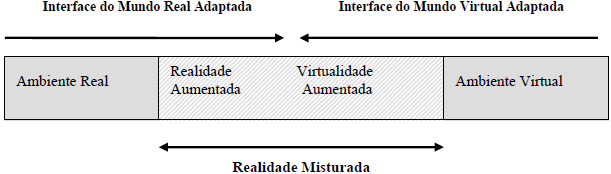
\includegraphics[scale=.8]{figuras/cap2/rv.jpg}
		\caption{\textit{Ambiente de Realidade Misturada ~\cite{kernerTori}}}
		\label{fig:diagramaRV} 
	\end{figure}
	
	\begin{enumerate}
	  \item \textbf{Ambiente Real:} Representa um ambiente constituído exclusivamente de objetos reais. 
	
	  \item \textbf{Realidade Aumentada:} Possui o ambiente real como interface de interação com o
	  usuário, com o propósito de inserir novas informações nele através de objetos virtuais.

	  \item \textbf{Virtualidade Aumentada:} A diferença entre a Realidade Aumentada e a Virtualidade
	  Aumentada está em sua forma de interação. Esta tem a finalidade de inserir elementos reais dentro
	  do mundo virtual e utilizar o ambiente virtual como interface de usuário. Para que isso ocorra, a
	  Virtualidade Aumentada utiliza técnicas computacionais para capturar elementos reais e inseri-los
	  no mundo virtual como objetos virtuais, como por exemplo, uma foto do usuário (objeto real) ser 
	  escaneada ou retirada através de uma~\textit{webcam} e ser inserida no mundo virtual para compor o
	  objeto virtual.

	  \item \textbf{Ambiente Virtual:} É definido como um ambiente compostos exclusivamente por objetos
	  virtuais, simulando um ambiente completamente sintético.
	
	\end{enumerate}
	
	Como um todo, os sistemas desenvolvidos para a Realidade Aumentada apresentam pontos chaves para
	seu funcionamento~\cite{henrysson}:
	
	\begin{enumerate}
	  \item \textbf{Rastreamento:} O sistema é responsável por obter as informações corretas a respeito
	  do posicionamento e orientação do usuário. A recuperação dessas informações torna-se necessária
	  		para a apresentação do conteúdo virtual correspondente. Nesta etapa são utilizados equipamentos
	  		(seção~\ref{sec:equipamentos}) responsáveis pela captura e processamentos dessas informações. O
	  		estabelecimento desses parâmetros é conhecido como \textit{tracking}. 
	  
	  \item \textbf{Registro:} Após o rastreamento ser concluído é feito o registro das informações
	  		correspondente a cada objeto reconhecido. O registro deve ser feito de modo que seja
	  		preservada a interatividade do usuário para que a relação entre o real e o virtual estejam
	  		alinhadas dentro de um mesmo domínio.
	  			
	  \item \textbf{Visualização:} A partir do resultado final gerado, esse sistema deve ser capaz de
	  produzir os objetos correspondentes em algum dispositivo que permita ao usuário visualizar tais
	  		informações.
	  
	\end{enumerate}
	
	O processamento destas imagens é constituído de etapas bem definidas
	(seção~\ref{sec:reconhecimentoMarcadores}), tendo como etapa inicial o reconhecimento dos
	marcadores utilizados pela Ralidade Aumentada e, posteriormente, a obtenção do código
	identificador do marcador. Por fim, a construção do objeto virtual correspondente.
	
	\section{Aplicações}
\label{sec:aplicacoes}

	Tendo em vista o potencial de aplicação da Realidade Aumentada na interação com usuários muitos estudos tem
	sido realizados neste sentido. Aplicações tem sido desenvolvidas em diversos ramos da atividade humana. 
	A seguir exemplifica-se alguns usos da Realidade Aumentada:
	
	\begin{itemize}
	  \item \textbf{Entretenimento} 
	  
	  		É nessa área que encontra-se o maior número de aplicações utilizando a Realidade
	  		Aumentada, sendo estas desenvolvidas principalmente para a área de jogos. O grande
	  		diferencial em utilizar a Realidade Aumentada em jogos é fazer com que seus cenários interajam
	  		com o mundo real ao qual o usuário está inserido. Isso possibilita uma interação maior
	  		do usuário e o cenário apresentado pelos jogos. 
	  		
	  \item \textbf{Medicina} 
	  
	  		O uso da Realidade Aumentada vem auxiliando a medicina em muitos aspectos, desde a visualização
	  		partes do corpo até a sua utilização em cirurgias. O \textit{HMD (Head Mounted Display)} é um
	  		equipamento bastante utilizado para auxiliar na visualização dos objetos virtuais,
	  		possibilitando que o mesmo seja seja utilizado em cirurgias guiadas por imagens. Deste modo,
	  		essa aplicação da Realidade Aumentada auxiliará em um melhor planejamento cirúrgico,
	  		contribuindo para uma diminuição dos riscos envolvidos~\cite{suthau, nilsson}.
	
	  \item \textbf{Mercado imobiliário e arquitetura} 
	  
	  		Maquetes e \textit{design} de interiores são construídas utilizando Realidade Aumentada com
	  		propósito de exemplificar aos consumidores o estado do empreendimento ao término de sua
	  		construção. Desta forma, a Realidade Aumentada é bastante utilizada nessas áreas para
	  		possibilitar aos compradores visualizar e customizar seus ambientes, possibilitando a
	  		modificação da disposição dos objetos e a observação dessas novas disposições.
	  		%com que o comprador faça modificações nas disposições dos objetos do jeito que achar
	  		% necessário e observar suas novas disposições.

	  \item \textbf{Auxílio na obtenção de informações a respeito de produtos} 
	  
	  		Empresas utilizam a Realidade Aumentada com o propósito de oferecer maiores detalhes a respeito
	  		de seus produtos. Eles são identificados por marcadores reconhecidos pela Realidade Aumentada.
	  		As informações necessárias são extraídas após o reconhecimento desse marcador e um objeto
	  		virtual contendo informações a respeito do produto é apresentado ao usuário. No caso de uma
	  		rede de supermercados, tais informações poderiam representar descontos, opiniões e ingredientes
	  		de produtos anunciados. Utilizando ainda o exemplo anterior, a localização dos produtos dentro
	  		do estabelecimento poderia ser mapeada de uma forma com que uma aplicação pudesse auxiliar o
	  		usuário a encontrar um determinado produto, através de uma navegação guiada por GPS
	  		ou por outros marcadores que guardariam a localização referentes a cada tipo de produto.
			
							  		
	  		%A visualização 3D do conteúdo interior de um produto a partir de marcadores posicionados nas
	  		%caixas do produto, proporcionou empresas utilizarem a realidade aumentada para possibilitar
	  		% com que os clientes possam obter maiores detalhes sobre o produto antes da compra.
	  
	  %%TODO arrumar a referência Augmented Reality Technology for Education, Mariano Alcatriz
	  % (procurar o bibtex)
	  \item \textbf{Educação}  
	  
	  		Através dos benefícios providos pela flexibilidade e usabilidade, a Realidade
	  		Aumentada foi utilizada na educação com o foco na aprendizagem. Sua utilização vai
	  		além da aprendizagem utilizando somente os livros, ela explora características que até então
	  		não eram percebidas no ambiente acadêmico, potencializando sua aprendizagem devido
	  		principalmente a interatividade provida pela Realidade Aumentada
	  		\cite{kaufmann,markBillinghurst}. Para exemplificar essa aplicação na Realidade Aumentada, 
	  		objetos dentro do museu britânico foram mapeados utilizando marcadores reconhecidos pela
	  		Realidade Aumentada proporcionando aos visitantes obterem informações a respeito dos objetos
	  		apresentados~\cite{museum}. Por outro lado, a Realidade Virtual vem sendo aplicada na educação
	  		desde a década de 90. Esses projetos proporcionam a criação de um mundo virtual com o propósito
	  		de ensinar e investigar os aspectos relacionados, como por exemplo, da cinemática,
	  		eletrostática, estruturas moleculares, estudo da biologia e matemática~\cite{ko, hannes}.
			
	  %% ~\cite{mariano}
	
	  \item \textbf{Turismo} 
	  
	  		Essa área tem sido bastante explorada devido a possibilidade de mapeamento de pontos
	  		turísticos e disponibilização de informações através desse mapeamento. Essas informações podem
	  		ser disponibilizadas de acordo com o perfil do usuário, com objetivo de auxiliá-lo na busca de
	  		locais de seu interesse. A localização desses pontos é feito através das coordenadas de
	  		localização do usuário, obtidas através de um GPS. Essas informações são cruzadas com posições
	  		de longitude, latitude e altitude obtidas de um banco de dados contendo todos os mapeamentos
	  		feitos. Na Realidade Aumentada essas posições mapeadas são denominadas de POI's (\textit{Points Of
	  		Interest}). Por causa da mobilidade obtida por esses recursos, eles são encontrados
	  		principalmente em aplicações voltadas para dispositivos móveis.
	
	\end{itemize}
	
	
	Como observado, a Realidade Aumentada é utilizada em diversas áreas com base em uma característica
	comum entre elas, a possibilidade de interação entre o real e o virtual. A visualização dos recursos
	providos pela Realidade Aumentada necessita de equipamentos compatíveis. Esses equipamentos
	proporcionam a captura de imagens, correspondente ao ambiente real do usuário, a construção e
	apresentação de objetos virtuais ao usuário.
	

	\section{Equipamentos}
\label{sec:equipamentos}

	Como etapa inicial para o funcionamento da Realidade Aumentada, necessita-se de equipamentos que
	possuam a funcionalidade de captura de vídeo, como por exemplo~\textit{webcam's}. Esses
	proporcionam a captura do ambiente do usuário e envia os dados para um dispositivo responsável pelo
	processamento. Dentre os equipamentos utilizados inicialmente na Realidade Aumentada pode-se citar
	o~\textit{HMD (Head Mounted Display)}. Eles eram utilizados com o objetivo de captura das
	informações, através de suas câmeras acopladas, posteriormente processavam as informações
	necessárias e exibia o resultado do processamento ao usuário através de objetos virtuais
	visualizados em suas telas acopladas ao equipamento.
	
	Este equipamento é fixado na cabeça do usuário podendo ter o formato de um capacete ou de um
	óculos. Algumas utilidades desse equipamento pode ser encontrada em realizações de simulações
	computadorizadas e também para a visualização dos objetos virtuais ao qual o âmbito da Realidade
	Aumentada está inserida~\cite{ronaldAzuma}.
		
	Quando esse equipamento foi proposto, ele possuía algumas desvantagens por ser muito pesado e
	evasivo. Atualmente, projetos estão sendo desenvolvidos para tentar minimizar essas desvantagens. A
	figura~\ref{fig:hmd} mostra um equipamento~\textit{HMD} com características que favoreçam sua
	utilização. Por outro lado, a grande vantagem desse tipo de equipamento é a possibilidade de
	imersão do usuário em um ambiente onde ele consiga interagir entre o virtual e o real de uma forma
	mais natural.
	
	\begin{figure}[htb]
		\centering 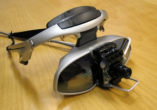
\includegraphics[scale=1.25]{figuras/cap2/hmd.jpg}
		\caption{\textit{Head Mounted Display ~\cite{nilsson}.}}
		\label{fig:hmd} 
	\end{figure}
	
	Atualmente, os \textit{smartphones} estão ganhando cada vez mais espaço dentro da Realidade
	Aumentada. Com a evolução do \textit{GPU (Graphics Processing Unit)} nestes, ocorreu a
	popularização de seu uso em aplicações voltadas para a Realidade Aumentada. A grande vantagem em
	sua utilização está na abrangência com que eles são distribuídos e principalmente na mobilidade
	conseguida através dos mesmos. Este equipamento comporta todos os recursos necessários para sua
	utilização na Realidade Aumentada:
	
	\begin{enumerate}
	  	\item A câmera do celular substitui a \textit{webcam} ou as câmeras acopladas ao HMD;
		\item O processamento gráfico é feito na~\textit{GPU};
		\item O resultado é apresentado no próprio visor do aparelho, suprindo a necessidade de um
		monitor ou telas para a visualização do objeto virtual.
	\end{enumerate}

	Um exemplo de utilização da Realidade Aumentada em \textit{smartphones} pode ser visto na
	figura~\ref{fig:arAndroid}. Nesta, a câmera do \textit{smartphone} captura a imagem do marcador,
	processa as informações necessárias e exibe um carro como objeto virtual correspondente para aquele
	marcador.
						
	\begin{figure}[htb]
		\centering 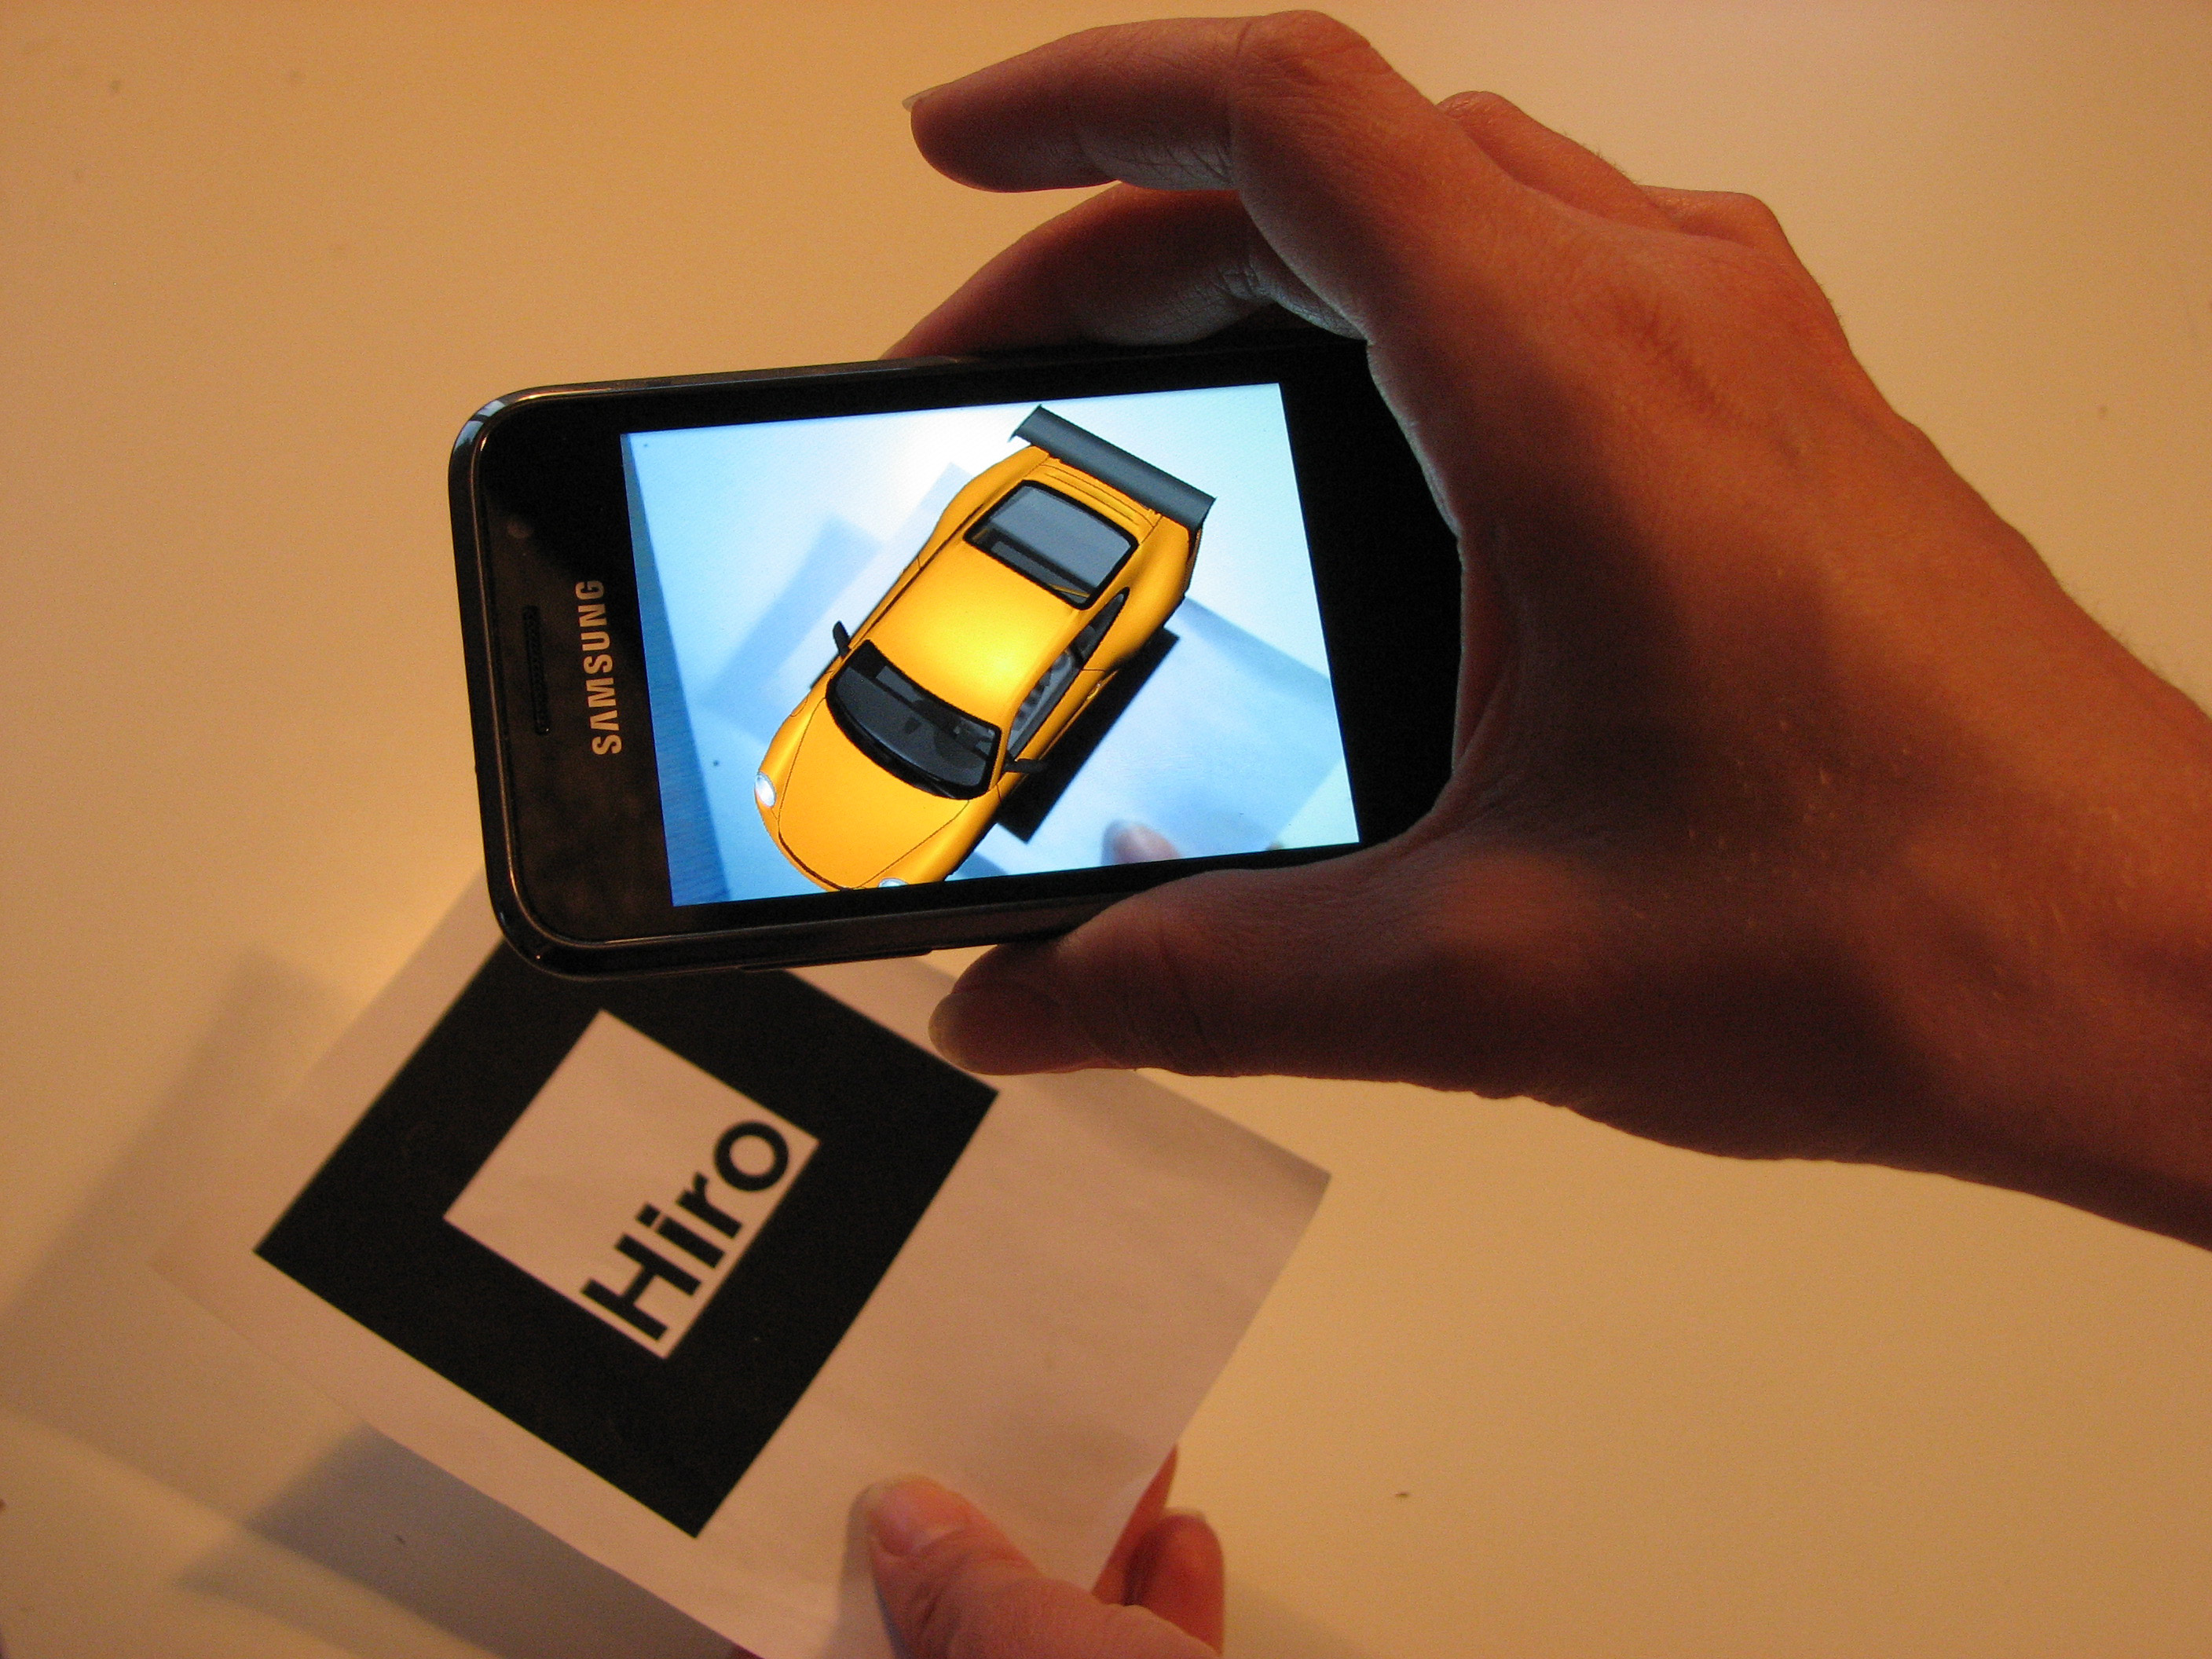
\includegraphics[scale=0.1]{figuras/cap2/ARToolKit-car-Android.jpg}
		\caption{\textit{Exemplo de utilização de smartphone na Realidade Aumentada~\cite{arToolWorks}.}}
		\label{fig:arAndroid}
	\end{figure}
	\section{Classificação}
\label{sec:classificacao}
	
	Com a evolução dos equipamentos, a visualização dos objetos virtuais torna-se cada vez mais real.
	Através desses equipamentos, os sistemas de Realidade Aumentada podem ser classificados de acordo
	com a forma como que o usuário vê o mundo misturado. Em~\cite{ronaldAzuma} é apresentado uma
	divisão para classificações entre as tecnologias óptica e vídeo. Essas classificações variam de
	acordo com o tipo de equipamento utilizado e com o tipo de sistema de visualização:
	
	\begin{enumerate}
		\item \textbf{Visão direta}
		
		Também conhecida como visão imersiva, nesta classificação os objetos virtuais são visualizados
		na mesma direção com que as cenas reais são capturadas. Esta classificação é utilizada
		principalmente em equipamentos que capturam as imagens reais, processam as informações
		necessárias e apresentam objetos ao usuário no mesmo equipamento~\cite{suthau}. Por
		exemplo, a utilização de equipamentos do tipo \textit{HMD} proporciona ao usuário uma visão
		direta, tendo em vista que a captura das cenas e a apresentação do objeto virtual foi feito pelo
		mesmo equipamento. Desta forma o usuário não necessita desviar o foco do mundo real a fim de
		observar as informações providas pelo objeto virtual.
		
		%Isso proporciona com que o usuário não precise desviar o olhar para a visualização do objeto
		% virtual.
		
		\item \textbf{Visão indireta}
		
		Ocorre quando a visualização do mundo misturado é feita através de algum dispositivo e a
		apresentação dos objetos virtuais, correspondentes as cenas, seja feita em um outro dispositivo,
		ocasionando o desvio da atenção do usuário~\cite{suthau, kernerTori}. Um exemplo para
		esse tipo de classificação é observado quando a captura das imagens reais é feita através de uma
		\textit{webcam}, processadas em um computador e o resultado apresentado em projeções ou em
		monitores.
		
	\end{enumerate}
	
	Uma outra forma de se classificar a Realidade Aumentada baseia-se nos sistemas utilizados por ela.
	Estes podem ser classificados de acordo com o tipo de equipamento utilizado para captura de cenas
	reais, processamento e os equipamentos responsáveis pela visualização do objeto virtual. Estas
	classificações abrangem tanto sistemas que utilizem visão óptica quanto visão por vídeo. Sendo
	classificados em:
		
	\begin{enumerate}
	
		\item \textbf{Visão direta por vídeo} 
		
		Neste tipo de classificação, equipamentos \textit{HMD} são utilizados para o recebimento direto
		da imagem real através de suas câmeras acopladas. As imagens capturadas são processadas em
		um gerador de cenas e as informações virtuais geradas por este são apresentadas diretamente ao
		usuário, através das telas acopladas ao equipamento. 
		
		%Nesta, um equipamento é utilizado para combinar cenas reais com as virtuais, a partir de
		%imagens obtidas através desse equipamento composto por pequenas câmeras de vídeo. As imagens
		%capturadas são processadas e novas informações virtuais são geradas por um computador. Essas
		%informações são misturadas com as cenas reais capturadas pelas micro câmeras acopladas ao
		%equipamento e as novas informações geradas pelo gerador de cenas são mostradas diretamente ao
		%usuário através das telas acopladas ao equipamento.
		
		\item \textbf{Visão direta por óptica} 
		
		De forma análoga a visão direta por vídeo, esta possui as mesmas etapas para obtenção e geração
		as informações virtuais a serem apresentadas ao usuário. No entanto, as informações geradas são
		apresentadas ao usuário através de lentes ou espelhos. Estas são inclinadas e posicionadas
		para que a projeção das imagens vindas do monitor acoplado seja refletida e redirecionada para
		os olhos do usuário.
		
		\item \textbf{Visão por vídeo baseada em monitor} 
		
		Após a captura das cenas, os objetos virtuais são gerados no gerador de cenas e misturados com
		as cenas reais no combinador de cenas. As informações geradas são apresentadas ao usuário
		através de um monitor.
		
		\item \textbf{Visão por óptica baseada em projeção} 
		
		Nessa classificação, as imagens dos objetos virtuais são apresentadas sem a necessidade de um
		equipamento específico. As mesmas são processadas em computador e projetadas em superfícies do
		ambiente real, por causa da necessidade de superfícies específicas para projeções, essa
		classificação torna-se mais restrita em comparação com as demais classificações.
		
	\end{enumerate}

	\section{Marcadores}
\label{sec:marcadores}

	Atualmente, é possível encontrar aplicações que utilizam padrões de símbolos bidimensionais para
	compor informações e transportar as mesmas de uma forma mais simplificada, a exemplo dos
	padrões~\textit{QRCode, PDF147} e~\textit{DataMatrix}~\cite{gao}. Alguns padrões permitem que as
	informações estejam representadas de forma redundante, pois auxiliam em sua detecção e na correção
	de possíveis erros. No âmbito industrial, seu campo de aplicação varia de acordo com a necessidade
	de cada sistema, como por exemplo transportar informações em etiquetas. Outros tipos de marcadores
	são utilizados para representar dados de localização e reconhecimento de objetos, como visto na
	Realidade Aumentada.
	
\subsection{Símbolos bidimensionais}
	\label{sec:simbolos_bidimensionais}
	
	Esse tipo de código de barras foi desenvolvido por volta de 1987. No código de barras bidimensional
	as informações são armazenadas tanto na altura quanto na largura, por essa razão possui uma maior
	capacidade de armazenamento das informações quando comparada aos símbolos unidimensionais. Os
	modelos de códigos unidimensionais armazenam as informações em apenas em uma dimensão, por
	causa dessa característica há uma limitação na quantidade de informação ser armazenada
	por eles, de acordo com cada padrão.  
	
	Para exemplificar essas características é apresentada a figura~\ref{fig:simbolos} ilustrando
	esses dois tipos de símbolos. O código apresentado na figura~\ref{fig:barcode} corresponde a um
	símbolo unidimensional, a altura desse símbolo (representado no eixo vertical) fornece
	redundância e legibilidade, possibilitando um tempo de resposta rápida, uma vez que a análise é
	feita em uma dimensão. Devido a limitação no armazenamento das informações por ele, geralmente são
	guardados valores chaves que possibilitem a busca de informações correspondentes ao código em um
	banco de dados específico. A figura~\ref{fig:datamatrix} apresenta um símbolo bidimensional
	denominado~\textit{DataMatrix}, as informações contidas neste são armazenadas em ambos os eixos
	horizontal e vertical, otimizando o espaço utilizado por ele, possibilitando a inserção de
	caracteres alfanuméricos, bem como um mecanismo responsável pela correção das informações obtidas
	através do processo de decodificação. Em contraste com esse modelo encontrado nos códigos
	unidimensionais, as informações armazenadas por esse símbolo remete a um conceito de banco de dados
	portátil e não somente o conceito de chave como apresentado no modelo unidimensional, podendo 
	armazenar uma maior quantidade de informação~\cite{gao}.
	
	\begin{figure}[htb]
		\centering
			\subfloat[\textit{BarCode} \cite{ean13}]{
				\label{fig:barcode}
				\centering 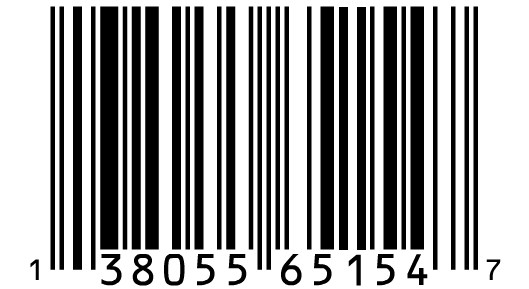
\includegraphics[scale=0.3]{figuras/cap2/codigo_barras.jpg}
			}
			\subfloat[\textit{DataMatrix} \cite{gao}]{
				\label{fig:datamatrix}
				\centering 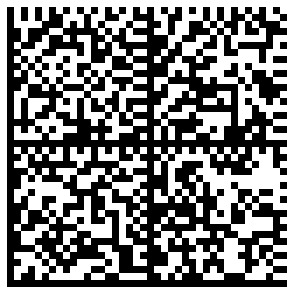
\includegraphics[scale=0.4]{figuras/cap2/datamatrix.jpg}
			}
		\caption{\textit{Exemplos de símbolos unidimensional e bidimensional.}}
		\label{fig:simbolos} 
	\end{figure}
	
	Os códigos bidimensionais podem ser divididos em duas categorias. A primeira denominada
	~\textit{stacked code} e a segunda chamada de~\textit{matrix code}. A diferença entre essas
	categorias está na sua composição. Enquanto que a~\textit{stacked code} trabalha com simbologias
	compostas por uma série de código de barras unidimensionais empilhadas uma em cima das outras,
	a~\textit{matrix code} codifica os dados com base nas posições dos pontos negros definidos dentro
	de uma matriz. Isso faz com que cada elemento da matriz possua a mesma dimensão, desta forma a
	decodificação é calculada em relação a posição do elemento preenchido na matriz. A
	tabela~\ref{tab:exemplo} apresenta alguns tipos de códigos bidimensionais e a categoria
	correspondente a cada código listado.
	
	
	\begin{table} % aqui começa o ambiente tabela
		\centering
		\caption{Códigos bidimensionais e suas categorias.}
		\begin{tabular}{lcc} 
			\hline % este comando coloca uma linha na tabela
			\textbf{Código bidimensional} & \textbf{Categoria} \\ 
			%\textit{\textbf{Stacked code}} & \textit{\textbf{Matrix code}}	\\
			\hline
			\hline
			\textit{Code 49} & \textit{Stacked} \\
			\textit{Data Matrix} & \textit{\textit{Matrix}} \\
			\textit{Portable Data File 417 (PDF417)} & \textit{Stacked}  \\
			\textit{QRCode} & \textit{\textit{Matrix}}\\
			\hline
		\end{tabular}
		\label{tab:exemplo}
	\end{table}
	
	A figura \ref{fig:qrCode} exemplifica um código de barras bidimensional da 
	categoria~\textit{matrix code}. Esse tipo de código é denominado de \textit{QRCode (Quick Response Code)}. 
	O \textit{QRCode} foi desenvolvido no Japão, no ano de 1994 com o objetivo de ser um código que possibilitasse um
	bom armazenamento de informações, compacto e que oferecesse uma leitura rápida e de fácil acesso.
	Este código pode codificar até 7089 caracteres numéricos (somente números), 4296 caracteres alfanuméricos 
	(letras e caracteres ASCII) ou 2953 \textit{bytes} de dados binários (\textit{bytes} hexadecimal)~\cite{kato}. Possui um 
	formato quadrático com dimensões variando
	de 21 x 21 até 177 x 177 células (conforme a versão do~\textit{QRCode}), onde cada célula codifica
	um \textit{bit}. É oferecido quatro níveis de detecção e correção de erros, possibilitando a
	recuperação de informações de regiões danificadas do código. A tabela~\ref{tab:nivelFalha}
	exemplifica esses níveis e apresenta a porcentagem de recuperação das informações oferecida por
	cada nível.
	
	
	\begin{table}
		\centering
		\caption{Níveis de correção de erros suportado pelo QRCode~\cite{kato}.}
		\begin{tabular}{lcc} 
			\hline
			 \textbf{Nível} & \textbf{Porcentagem de informação recuperada} \\
			\hline
			\hline
			\textit{Low} & 7\% \\
			\textit{Medium} & 15\% \\
			\textit{Quality} & 25\% \\
			\textit{High} & 30\% \\
			\hline
		\end{tabular}
		\label{tab:nivelFalha}
	\end{table}
	
	
	O \textit{QRCode} possui características estruturais com o objetivo de facilitar sua identificação
	e obtenção das informações necessárias para a sua correta decodificação. Tais características
	estão ilustradas na figura~\ref{fig:qrCode}.
				
	\begin{figure}[htb]
		\centering 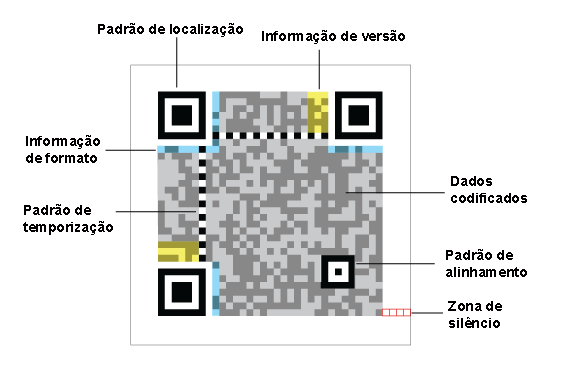
\includegraphics[scale=0.6]{figuras/cap2/qranatomy.png}
		\caption{\textit{Ilustração das propriedades estruturais do QRCode. Adaptado de~\cite{qrcodespec}.}}
		\label{fig:qrCode} 
	\end{figure} 
	
	\begin{itemize}
	  \item \textit{Padrão de localização}
			  
	  	Esse padrão baseia-se nas posições dos três vértices localizadas nos cantos do símbolo. A
	  	partir desses três pontos é possível estimar o quarto canto da imagem, por consequência a
	  	posição, tamanho e o centro dos símbolos podem ser detectados, sendo assim utilizado para
	  	referência posicional do símbolo. Desta forma, o reconhecimento pode ser feito em todas as
	  	direções.
				  
		\item \textit{Padrão de temporização}
				  
		Padrão responsável pela identificação e correção das coordenadas centrais de cada célula. Este
		padrão é utilizado quando o símbolo está distorcido, possibilitando a identificação do espaçamento
		entre as células.
					
		\item \textit{Padrão de alinhamento}
					
		Por fim, a correção de distorção, especialmente a não linear, é feita através desse padrão. 
		Essa visa corrigir a distorção do símbolo quando este estiver em uma superfície curva ou 
		com o leitor inclinado.	Por fim, esta célula facilita a obtenção da coordenada central do padrão 
		de alinhamento.
		
		\item \textit{Dados codificados}
		
		É a região responsável pelo armazenamento dos dados codificados.
		
		\item \textit{Informação de formato}
		
		Contém a taxa de correção de erro e o padrão de máscara utilizado.
		
		\item \textit{Zona de silêncio}
		
		É a margem ao redor do \textit{QRCode} necessário para que o código seja lido corretamente. Possui
		a medida correspondente a quatro células de largura.
		
		\item \textit{Informação de versão}
		
		Responsável pela identificação da versão utilizada pelo \textit{QRCode}, podendo variar a partir
		da versão 1 (correspondente a 21 x 21 células) até a versão 40 (correspondente a 177 x 177
		células). As versões possuem a mesma estrutura, porém a capacidade de armazenamento varia de uma
		versão para outra.
									
	\end{itemize}
	
	A tabela \ref{tab:tabelaCodigos} mostra um comparativo entre diferentes tipos de códigos tanto
	unidimensionais (\textit{barcode}) quanto bidimensionais (\textit{QRCode} e \textit{Data Matrix}).
	As quantidade de referência internas apresentadas na tabela dizem respeito a pontos contidos
	internamente dentro do código cujo propósito seja o auxílio para obtenção do correto
 	posicionamento do mesmo. Também é mostrada a diferença na quantidade de informação armazenada por
	esses códigos.
	
	
	\begin{table} % aqui começa o ambiente tabela
		\centering
		\caption{Comparação de vários códigos \cite{marlon}.}
		\begin{tabular}{lccc} 
			\hline % este comando coloca uma linha na tabela
			 & \textbf{\textit{Barcode}} & \textbf{QRCode} & \textbf{\textit{DataMatrix}} \\
			\hline
			\hline
			Capacidade de armazenamento & 1\textit{byte}/4cm	 & 2953 \textit{bytes} & 2335 \textit{bytes} \\
			Velocidade de leitura & Rápido & Rápido & Lenta\\
			Especificação aberta & Sim & Sim & Sim\\
			Referências internas & 0 & 3 & 2 \\ 
			Recuperação dos dados & Não & Até 30 \%  & Até 30 \% \\
			Formato & Linear & Quadrado & Retangular\\
			\hline
		\end{tabular}
		 % igual ao ambiente figura
		\label{tab:tabelaCodigos}
	\end{table}
	
\subsection{Marcadores para Realidade Aumentada}
\label{sec:marcadoresRA}
		
		Cada aplicação voltada para a criação e/ou detecção de marcadores pode possuir seus próprios
		padrões de marcadores e algoritmos para seu reconhecimento. A área de definição de marcadores
		utilizados ainda está em aberto, com espaço para melhorias de acordo com cada aplicação~\cite{fpga}. Dentro
		desse universo pode-se citar as aplicações ARToolkit~\cite{artoolkit}, ARTag~\cite{artag} e
		ARToolkitPlus~\cite{kler}.
		
		De uma forma geral, para os objetos sejam reconhecidos como potenciais marcadores por
		essas aplicações, estes necessitam de um formato padrão constituído por uma ``moldura''
		confeccionada com bordas quadradas, de preferência na cor preta, pois algumas aplicações convertem
		as cores da imagem em uma escala de cinza. A construção e decodificação do conteúdo interior do
		marcador pode variar de acordo com cada aplicação, possibilitando uma flexibilização na construção
		do mesmo. Na abordagem da aplicação ARToolkit, o centro desses marcadores pode ser constituído por
		uma figura. Já no ARToolkitPlus, o interior dos marcadores é preenchido por quadrados de cor
		preta, podendo formar figuras geométricas diversas. Exemplos de marcadores utilizados por essas
		aplicações são apresentados na figura~\ref{fig:marcadoresAR}. 
		
		\begin{figure}[htb]
			\centering
				\subfloat[ARToolKit \cite{artoolkit}]{
					\label{fig:artoolkit}
					\centering 
\includegraphics[scale=1]{figuras/cap2/arToolkitMarker.png}
				}
				\subfloat[ARTag \cite{artag}]{
					\label{fig:artag}
					\centering 
\includegraphics[scale=1]{figuras/cap2/arTagMarker.png}
				}
				\subfloat[ARToolkitPlus \cite{kler}]{
					\label{fig:artoolkitplus}
					\centering 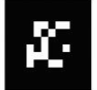
\includegraphics[scale=1]{figuras/cap2/arToolkitPlusMarker.png}
				}
			\caption{\textit{Exemplo de alguns marcadores utilizados na realidade aumentada.}}
			\label{fig:marcadoresAR} 
		\end{figure}
		
	Fazendo uma comparação entre esses marcadores e o \textit{QRCode} é possível observar que, da mesma
	forma como acontece com o código unidimensional apresentado na tabela~\ref{tab:tabelaCodigos},
	estes não possibilitam a recuperação de informações danificadas, mas possibilitam a identificação do erro. 
	Desta forma o não reconhecimento de parte do marcador pode comprometer todo o processo de reconhecimento. 
	Diferentemente do \textit{QRCode}, esses marcadores possuem uma capacidade bastante limitada para 
	armazenamento de informações. Por causa dessa limitação a maioria dos marcadores guardam somente um código
	identificador. Entretanto, são menos sensíveis a distorções de ângulo devido sua simplicidade. 
	

	\section{Reconhecimento de marcadores}
\label{sec:reconhecimentoMarcadores}	
	
		O processo de reconhecimento dos marcadores é dividido em etapas bem definidas. No entanto, estas
		podem ser implementadas de formas diferentes levando-se em consideração a aplicação utilizada.
		Esse processo tem o objetivo de identificar objetos com formatos pré-definidos e que possuam
		códigos de identificação compatíveis com a aplicação. A partir desse
		reconhecimento é possível estabelecer o posicionamento dos objetos em relação ao dispositivo
		responsável pela captura da imagens e apresentar o objeto virtual correspondente sobreposto ao
		marcador reconhecido. As etapas envolvidas nesse processo são apresentadas na
		figura~\ref{fig:pipelineAR} e dividas da seguinte maneira:
		
		\begin{figure}[htb]
			\centering 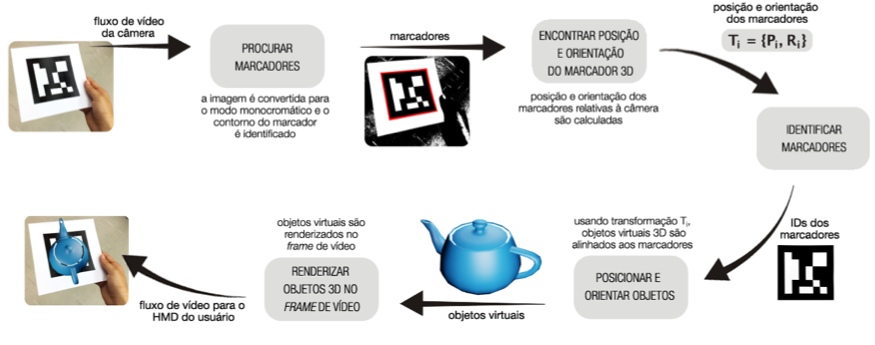
\includegraphics[scale=.55]{figuras/cap2/pipelineAR.png}
			\caption{\textit{Etapas do processo de reconhecimento de marcadores na Realidade
			Aumentada~\cite{fpga}.}}
			\label{fig:pipelineAR} 
		\end{figure}
		
		\begin{enumerate}
		  \item \textbf{Procurar marcadores}
		  
				O fluxo de vídeo obtido por uma câmera é entrada da etapa inicial do processo de
				reconhecimento. Ele é lido e encaminhado para o sistema de rastreamento. Neste, aplica-se uma
				operação de detecção de bordas como uma etapa inicial. Faz-se um reconhecimento de
				cada~\textit{pixel} dentro de um segmento para que seja feita um agrupamento de~\textit{pixels},
				a fim de se achar uma forma quadrangular e reconhecer a figura como um possível marcador. Esse
				método acaba sendo mais eficaz quando comparado com o método de derivar o marcador a partir de
				uma intensidade de luminosidade de escala de cinza, devido o seu reconhecimento em ambientes de
				pouca luminosidade e problemas relacionados com oclusão (parte da visualização do marcador é
				obstruída por um outro objeto)~\cite{artag}.
				
			\item \textbf{Encontrar posição e orientação do marcador 3D}
			
				Nesta etapa o marcador já foi encontrado na imagem. Para obter uma estimativa da posição do
				marcador é necessário obter quatro pontos não lineares e identificáveis na imagem. Estes pontos
				devem aproximar a um formato correspondente a um quadrado. Na situação de identificação das
				posições baseados na utilização de várias câmeras, envolve a localização do mesmo recurso em
				duas imagens obtidas por câmeras diferentes. Isso possibilitaria estimar a posição geométrica
				tridimensional de um recurso. Neste caso para estimar a localização de tal recurso necessitaria
				combinar as informações de três pontos não lineares. Alguns problemas podem ser detectados, como
				por exemplo, a distorção de perspectiva ocorrendo quando o plano da tela não é o mesmo plano do
				marcador~\cite{kler}.
				
			\item \textbf{Identificar marcadores}
			
				É nesta etapa que acontecem mais particularidades para o reconhecimento dos marcadores
				observadas em diferentes aplicações. Na aplicação ARTag, o conteúdo extraído do interior do
				marcador é preenchido com uma matriz quadrada 6 x 6 com células de cores preto e branco, aos
				quais representarão valores binários de 0's e 1's. Essa matriz retornará uma sequência de
				36~\textit{bits}, sendo analisada de quatro formas distintas por causa das quatro rotações
				possíveis para o marcador.
				
				O código identificador do marcador é constituído por 10 \textit{bits}, sendo codificado a
				partir da sequência dos 36~\textit{bits} obtidos e deixando os 26~\textit{bits} restantes para a
				detecção e correção de erros, bem como a unicidade em torno das quatro possibilidades de rotação
				do marcador~\cite{hirzer}. São utilizados os métodos~\textit{CRC (Cyclical Redundancy Check)}
				e~\textit{Forward Error Correction} para detecção do marcador e extração do seu número
				identificador correspondente, adicionando o conceito dos operadores lógicos XOR para codificação
				e decodificação. A correção e reparo dos erros, desalinhamento de fronteira, oclusão, dentro
				outros, fica sobre a responsabilidade do~\textit{FEC (Forward Error Correction)}. Outros
				métodos, baseados em probabilidades, também são aplicados para garantir o reconhecimento correto
				do identificador do marcador em relação aos demais marcadores.
				
				A figura \ref{fig:artagDecoding} exemplifica os passos necessários utilizado pelo ARTag para
				obter o código de identificação do marcador a partir do marcador reconhecido nas etapas anteriores 
				do~\textit{pipeline}.
				
				\begin{figure}[h]
					\centering 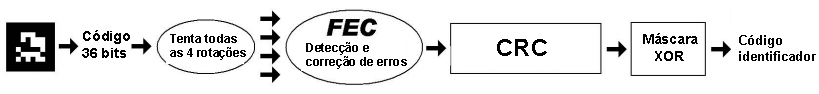
\includegraphics[scale=.55]{figuras/cap2/artag_decoding.png}
					\caption{\textit{Obtenção do código identificador do marcador. Adaptado de~\cite{artag}.}}
					\label{fig:artagDecoding} 
				\end{figure}
				
				De forma análoga, o ARToolkit extrai o conteúdo do interior do marcador e gera uma matriz
				quadrada. No entanto, as dimensões dessa matriz são de 16 x 16 ou 32 x 32. Os valores obtidos
				por essa matriz geram um vetor característico que é comparado com uma biblioteca de vetores
				característicos conhecidos e geram como resultado um fator de confiança para dizer se o
				marcador foi reconhecido.
				
			\item \textbf{Posicionar e orientar objetos}
			
				Nesta etapa, os objetos virtuais 3D são identificados e associados de acordo com o marcador
				identificado na etapa anterior. Os mesmos são alinhados ao marcador pelo posicionamento obtido na
				etapa 2.
			
			\item \textbf{Renderizar objetos 3D no ~\textit{frame} de vídeo}
			
				Por fim é gerado o \textit{frame} de vídeo, contendo o marcador e seu respectivo objeto virtual
				3D. Após ser renderizado, o mesmo é repassado para o objeto de visualização de vídeo, podendo ser um
				monitor,~\textit{HMD} ou \textit{smartphone}.
				
		\end{enumerate}
	
		A quantidade de marcadores, aos quais podem ser geradas com uma boa qualidade de reconhecimento
		varia para cada tipo de aplicação. Essa qualidade de reconhecimento refere-se a símbolos no
		interior dos marcadores aos quais são facilmente distinguíveis pelas aplicações. Isso mostra 
		que a quantidade de \textit{bits} obtidos a partir da matriz gerada pelo interior do marcador,
		pode-se construir diversos símbolos. No entanto, pela isomorfia dos marcadores (rotação do marcador 
		em 0, 90, 180 e 270 graus) muitos símbolos acabam sendo descartados por se tratar do mesmo marcador. 
		No ARTag e no ARToolkitPlus, esses números são bastantes diferentes.
		Enquanto que no primeiro, 2002 marcadores são reconhecidos facilmente, no segundo esse número cai
		para 512. Porem, muitos outros símbolos podem ser gerados, mas sem muita garantia de uma boa
		qualidade em seu reconhecimento. Não foi possível obter as mesmas informações a respeito da
		quantidade de marcadores que são reconhecidos pelo ARToolkit.
		
	
	
	\section{Trabalhos correlatos}
\label{sec:trabalhosRelacionados}

	O aumento da mobilidade no ambiente de trabalho de usuário, proporciona uma	abstração de diferentes 
	configurações de um ambiente, sendo suportado pelas diversas tecnologias de comunicação sem fio utilizadas na
	computação móvel. Desta maneira, vários trabalhos estão sendo desenvolvidos utilizando esta
	computação com o propósito de auxiliar o usuário na solução de seus problemas. Serão apresentados
	trabalhos que utilizam a computação móvel, aplicadas a ambientes ubíquo.
	 
	\subsection{\textit{CyberCode}}
\label{sec:cybercode}
	
	Em \cite{rekimoto} é apresentado uma proposta de utilização de marcadores baseados em códigos
	bidimensionais, denominado de CyberCode. Nesta aplicação as informações são codificadas em um
	padrão bidimensional para ser reconhecido por dispositivos de baixo desempenho. As informações
	correspondente aos marcadores são armazenados em um banco de dados, possibilitando assim a
	alteração dos dados de forma dinâmica, sem a necessidade de alterar o marcador. A
	figura~\ref{fig:cybercode} mostra um exemplo do marcador CyberCode.
	
	\begin{figure}[htb]
		\centering 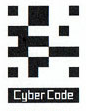
\includegraphics[scale=1]{figuras/cap2/cybercode.png}
		\caption{\textit{Exemplo de um marcador CyberCode \cite{rekimoto}.}}
		\label{fig:cybercode} 
	\end{figure} 
	 
	O uso dos mesmos pode ser combinado com outras tecnologias de rastreamento, com o objetivo de
	auxiliar o usuário na navegação em um ambiente específico. Desta maneira, eles seriam
	reconhecidos com o propósito de obtenção da localização do usuário no espaço. Com isso seria
	possível apresentar as informações ao usuário a respeito dos demais locais próximos a ele.
	
	Uma outra proposta para esses marcadores diz respeito a utilização dos mesmos para o mapeamento dos
	dispositivos. A própria equipe construiu um dispositivo de fácil manuseio constituído por uma
	câmera e um visor, denominado de \textit{InfoPoint}. Esse dispositivo capta a imagem correspondente
	ao marcador, acessa um banco de dados para extrair o conteúdo correspondente e apresenta o conteúdo
	correspondente no visor do dispositivo. Através desse dispositivo, o usuário é capaz de selecionar
	um marcador específico e transferir dinamicamente o conteúdo relativo a esse CyberCode para um outro
	marcador.
	
	\subsubsection{Aplicado à computação ubíqua}
	 
	A integração desse projeto com a computação ubíqua ocorre através da utilização de uma mesa
	digital. Sobre esta são acopladas câmeras com o propósito de reconhecer os objetos
	distribuídos em sua superfície. Após o reconhecimento de um novo dispositivo marcado por um
	CyberCode são apresentadas as informações correspondente ao objeto reconhecido. 
	
	Também é apresentada a utilização da mesa através da integração com um \textit{notebook}. O
	\textit{notebook} é reconhecido através do seu marcador associado, posteriormente é feita uma busca
	das informações relativas ao dispositivo, como por exemplo seu endereço~\textit{IP} e o
	posicionamento relativo a mesa digital. Desta forma, o \textit{notebook} estará integrado com a
	rede local juntamente com os objetos físicos reconhecidos pela mesa.
	
	Essa integração possibilita uma troca de informações livre entre os dispositivos. No exemplo
	anterior, o recurso de tela do \textit{notebook} foi estendido para a mesa digital. Isso
	possibilita com que o usuário utilize os recursos da mesa digital para interagir com o
	\textit{notebook}. Por exemplo, caso o usuário sinta a necessidade de mover o cursor do
	\textit{notebook}, ele poderá utilizar a sensibilidade da mesa para mover o cursor dentro do espaço
	delimitado como extensão da tela do \textit{notebook}.
	

	\subsection{\textit{HELLO}}
\label{sec:hello}

	O projeto HELLO (\textit{Handheld English Language Learning Organization}) integra os benefícios
	providos pela Realidade Aumentada, computação ubíqua e móvel com o objetivo de auxiliar na
	aprendizagem da língua inglesa~\cite{tsung}. Esse projeto utiliza a tecnologia denominada de
	\textit{m-learning (Mobile Learning)} para que os alunos tenham acesso a informação independente
	do local físico que eles estejam, flexibilizando e potencializando a aprendizagem. Seu conceito
	de~\textit{u-learning (Ubiquitous Learning)}, visa a possibilidade do usuário ser inserido em um
	ambiente onde ele tenha as informações de forma acessível e transparente, com o propósito de
	flexibilizar e tornar contínuo o processo de aprendizagem. Desta maneira, o usuário obtém
	vantagens providas pela~\textit{ubicomp}, tais como: acessibilidade, interatividade e sensibilidade
	ao contexto.
	
	O funcionamento do projeto HELLO é divido em subsistema servidor e um utilitário denominado
	\textit{u-Tools}. A aplicação servidor fica responsável pelo armazenamento das informações, tais
	como: materiais didáticos, aulas, banco de dados, provas, dentre outros. A \textit{u-Tools} foi
	desenvolvida para a plataforma utilizada pelos \textit{PDA's (Personal Digital Assistant)},
	proporcionando assim as funcionalidades de acesso do conteúdo oferecido pela aplicação servidor
	(através de uma comunicação \textit{Wifi}), a leitura dos códigos de barra bidimensionais e auxílio
	na comunicação dos usuários. A prova de conceito do projeto foi realizado em um colégio de ensino
	médio com o propósito de medição do nível de aprendizagem dos alunos ao término do projeto.
	
	\subsubsection{Uso da Realidade Aumentada}
	
	Durante uma etapa de aprendizagem, o estudante tinha que obter informações a respeito da execução
	de uma atividade. Ao se aproximar de uma sala de aula, o aluno percebe a existência de um código de
	barras bidimensional perto da sala. Obtendo as vantagens providas pelos códigos de barras
	bidimensionais, o projeto HELLO utiliza o QRCode para obtenção de informação, junto a seus
	servidores, a respeito da localização do usuário e provê o conteúdo correspondente. O aluno então
	captura a imagem contendo o marcador e a envia para o processamento nos servidores.

	Após o processamento, o servidor envia as informações correspondentes ao usuário (um tutor virtual
	e os diálogos são apresentados no PDA do usuário) utilizando a Realidade Aumentada. Esse tutor fica
	responsável pela prática da conversação de acordo com o nível de complexidade da zona que o usuário
	esteja. Caso o usuário tenha êxito na conversação, o mesmo é encaminhado para uma nova zona até que
	se complete o percurso. Um exemplo dessa interação pode ser visto na figura~\ref{fig:hello}.
	
	\begin{figure}[htb]
		\centering 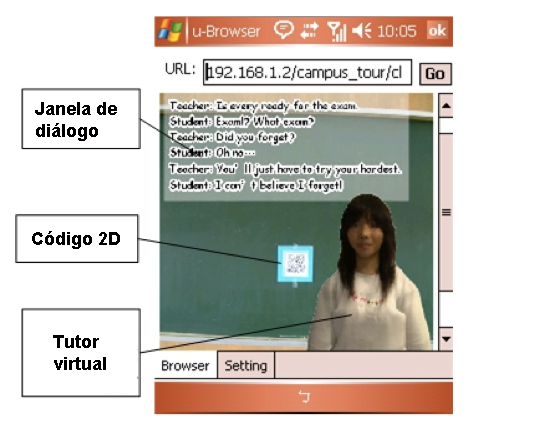
\includegraphics[scale=.7]{figuras/cap2/hello.png}
		\caption{\textit{Exemplo do tutor virtual utilizado no HELLO. Adaptado de~\cite{tsung}.}}
		\label{fig:hello} 
	\end{figure}
	\subsection{SmARt World}
\label{sec:smart}

	\textit{SmARt World} é um \textit{framework} voltado para a computação ubíqua, ao qual utiliza a 
	Realidade Aumentada com o objetivo de criar novos conteúdos virtual e interação com o ambiente
	inteligente~\cite{yew}. Outro objetivo desse \textit{framework} está no auxílio da construção de
	aplicações voltada para a Realidade Aumentada baseada em dispositivos móveis, tornando esse
	desenvolvimento simplificado. O \textit{framework} é capaz de criar e apresentar objetos virtuais
	ao usuário, provendo uma interação por meio destes. Sua arquitetura é dividida em: 
	
	%Sua arquitetura é ilustrada conforme a
	%figura~\ref{fig:arquitetura_smart}.
	
	%\begin{figure}[htb]
	%	\centering 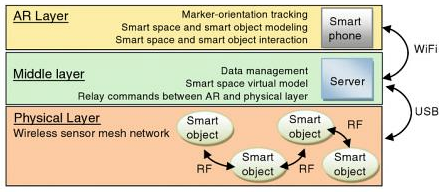
\includegraphics[scale=0.8]{figuras/cap2/arquitetura_smart.png}
	%	\caption{\textit{Arquitetura do framework SmARt World \cite{yew}.}}
	%	\label{fig:arquitetura_smart}
	%\end{figure}
	
	\begin{enumerate}
	  \item \textbf{Camada Física}
	  	
	  	Nessa camada os objetos inteligentes são interligados através de transmissores de rádio
	  	frequência, onde estes são ligados um nó central que faz acesso a Camada Intermediária. Esse nó
	  	central também fica responsável por reconhecer os demais nós ativos na rede, controlar as
	  	informações que são repassadas pelos nós e posteriormente enviar os dados a Camada Intermediária
	  	para que as informações correspondentes aos nós sejam atualizadas.
	  	
	  	Cada transmissor possui seu código identificador para se comunicar com a rede, essa comunicação
	  	é feita através de sensores ou por comunicações interligadas fisicamente. O objetivo da
	  	utilização desses transmissores acoplados aos dispositivos possibilita o controle dos
	  	mesmos, acrescentando uma inteligência a rede. Desta forma, de acordo com a informação captada
	  	pelos transmissores, é possível enviar sinais específicos para os dispositivos. Esse controle
	  	será feito através da interface provida pelo~\textit{smartphone}, na Camada AR.
	  
	  \item \textbf{Camada Intermediária}
	  
	  	Essa camada possui a responsabilidade de armazenar e gerenciar todas as informações a respeito
	  	do ambiente inteligente e dos usuários e objetos pertencentes a ele. A comunicação entre a
	  	aplicação e os demais componentes da rede é feita através de uma interface web que
	  	disponibiliza acesso a aplicação e ao banco de dados contido em servidor. O banco de dados
	  	armazena informação a respeito do objeto, tais como: posicionamento, modelagem 3D, textos
	  	apresentados ao usuário, formato e contexto. 
	  
	  \item \textbf{Camada AR}
	
		Essa camada utiliza uma aplicação voltada para a Realidade Aumentada que é capaz de
		rastrear e reconhecer os marcadores. Através disso possibilita uma interação entre os
		objetos virtuais e reais. Essa camada foi projetada para ser utilizada em dispositivos móveis.
		Por essa razão, o protótipo para essa camada foi desenvolvido para a plataforma Android.
		
	\end{enumerate}
	
	\subsubsection{Marcadores e a Realidade Aumentada}
	
	O rastreamento e reconhecimento dos marcadores é feito a partir de dois métodos combinados. O
	primeiro é o reconhecimento dos objetos através do uso de marcadores. Após o reconhecimento, o
	segundo método é iniciado. Neste, sensores são utilizados para obter a orientação e posicionamento
	do objeto. Esse posicionamento é gravado na Camada Intermediária através das coordenadas \{x,y,z\}. O
	\textit{framework} possui a funcionalidade de seleção de objetos virtuais através da tela do
	\textit{smartphone}, possibilitando redefinir o novo posicionamento do objeto virtual selecionado
	no ambiente inteligente.
	
	
	
	
	

	~\chapter{~\emph{ARHydra}}
\label{cap:arhydra}
	%\epigraph{`` The most profound technologies are those that disappear.''}{Mark Weiser}
	
		
	O \textit{smart space} pode ser composto por uma grande variedade de dispositivos, os quais
	disponibilizam recursos ao ambiente. Por sua vez, esses recursos devem ser utilizados para suprir
	as necessidades do usuário e auxiliar na execução de suas tarefas da melhor forma possível.
	Adicionalmente, o ambiente poderá oferecer ao usuário a possibilidade de seleção do recurso a ser
	utilizado na execução de uma tarefa. Dentro desse contexto, a aplicação Hydra (apresentado na
	seção \ref{sec:hydra}), utilizando o \textit{middleware uOS} (seção \ref{sec:uos}), possibilita ao
	usuário escolher e utilizar um determinado recurso disponível no ambiente.
	
	Devido a grande volatilidade e a quantidade de dispositivos dentro do ambiente inteligente, a
	aplicação ARHydra (apresentada na seção \ref{sec:arHydra}) utiliza os recursos providos pela
	Realidade Aumentada e os objetivos do \textit{uOS} auxiliando o usuário na visualização e seleção
	dos recursos presentes no ambiente inteligente.
	
	\section{O \textit{middleware} uOS}
\label{sec:uos}
	 
	O \textit{middleware uOS}, projeto do grupo de pesquisa \textit{UnBiquitous} da Universidade de
	Brasília, tem como objetivo a integração das aplicações no ambiente inteligente e foca na
	adaptabilidade dos serviços presentes nos mais diversos dispositivos. Desta forma, os serviços
	passam a ser compartilhados de uma forma menos intrusiva \cite{buzeto}. Conforme apresentado na
	figura~\ref{fig:dsoa}, o \textit{middleware uOS} atua como uma camada entre as aplicações
	e~\textit{drivers}.
	
	\begin{figure}[htb]
		\centering 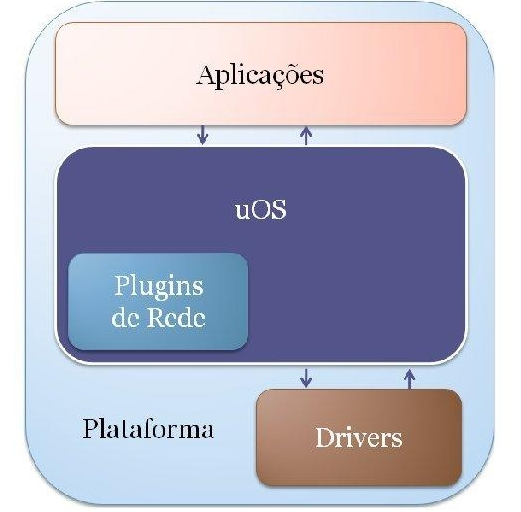
\includegraphics[scale=.35]{figuras/cap2/dsoa.jpg}
		\caption{\textit{Middleware uOS~\cite{buzeto}.}}
		\label{fig:dsoa} 
	\end{figure}
	 
	O \textit{uOS} segue os conceitos propostos pela ~\textit{DSOA} (\textit{Device Service Oriented
	Architecture}) para modelagem do ambiente inteligente. Nessa arquitetura são definidos o modelo
	de comunicação a ser utilizado, implementando algumas características definidas pelo
	~\textit{SOA (Service Oriented Architecture)}~\cite{buzeto_11}. Por causa da diversidade e capacidade de
	processamento dos diversos dispositivos presentes no \textit{smart space}, foi criado um conjunto
	de protocolos para a computação ubíqua, implementada sobre o ~\textit{middleware uOS}, denominada de ~\textit{uP
 	(Ubiquitous Protocols)}, viabilizando uma maneira simplificada e padronizada para a troca de
 	informações entre esses dispositivos. O \textit{uP} permite uma interação entre os dispositivos,
 	levando-se em consideração a heterogeneidade das plataformas, os diferentes modelos de comunicação
 	e interação com o ambiente. Desta forma, o \textit{uP} possibilita a descoberta de novos
 	dispositivos no ambiente e a representação dos recursos através de \textit{drivers}.
	
	O \textit{uOS} foi desenvolvido na linguagem JAVA, possibilitando a utilização do mesmo nos mais
	diversos dispositivos que a ofereçam suporte. Ele se encontra disponível em duas versões: uma
	\textit{mobile}, sob a plataforma JME (\textit{Java Micro Edition}), e uma seguindo a plataforma
	JSE (\textit{Java Standart Edition}). Esta última foi também portada para a utilização em
	dispositivos Android. Viabilizando sua utilização tanto em dispositivos limitados (usando a
	plataforma \textit{mobile} ou Android) à outros mais capazes.
	

	\section{A aplicação Hydra}
\label{sec:hydra}
	
	
	Na visão da \textit{ubicomp}, o \textit{smart space} é composto por diversos dispositivos que
	fornecem uma gama de recursos e funcionalidades. É plausível de se esperar que muitos destes
	recursos sejam equivalentes entre si, como a existência de várias telas a disposição. Com tantas
	opções espera-se que um ambiente inteligente possibilite ao usuário escolher aquela que melhor lhe
	atende na tarefa sendo realizada. É neste cenário que a aplicação Hydra entra em cena. Fazendo uso
	da plataforma provida pelo \textit{middleware uOS}, esta aplicação permite que o usuário
	redirecionar os recursos de sua máquina para outros mais adequados no ambiente \cite{almeida}.

    Para melhor entender a atuação da Hydra no ambiente considere o seguinte exemplo de uso:
	 
	O ambiente é dotado dos seguintes dispositivos:
	 
	
	\begin{enumerate}
		\item Macbook e o \textit{notebook} HP disponibilizam os recursos de \textit{webcam}, saída de
		vídeo, mouse e teclado;
		\item \textit{Laptop} Dell disponibiliza somente os recursos de saída de vídeo, mouse e teclado;
		\item \textit{Smartphone} Galaxy SII disponibiliza os recursos de câmera, mouse e teclado;
		\item \textit{SmartTV} disponibiliza os recursos de saída de vídeo. 
	\end{enumerate}
	
	A seguir temos um exemplo de interação neste ambiente utilizando a Hydra:

	\begin{quote}
	
		\it 	
		Inicia-se uma reunião cujo propósito é alinhar os conhecimentos a respeito dos projetos do grupo 
		UnBiquitous, discutir as soluções propostas e apresentar os artigos base para os projetos. Os
		participantes da reunião são Marcelo (dono do notebook HP), Bruno (dono do smartphone Galaxy SII), Ricardo (dono do
		Macbook) e Fabrício (dono laptop Dell).
		
		Para facilitar a visualização dos tópicos a serem discutidos, Fabrício como líder do projeto,
		instalou a aplicação Hydra em seu laptop e redirecionou a tela do laptop para a SmartTV. Os
		demais dispositivos estão utilizando uma instância do middleware uOS, disponibilizando seus
		recursos ao ambiente.

		Fabrício mostra a pauta da reunião. Após a discussão dos primeiros tópicos, Ricardo sente a
		necessidade de complementar alguns tópicos apresentados. Ricardo então pede ao Fabrício que
		redirecione o recurso de teclado do laptop Dell para seu Macbook. Após acrescentar os novos
		tópicos, Ricardo pede ao Fabrício que libere o recurso do teclado, para que seja utilizado o
		teclado do laptop do Fabríco novamente. Bruno percebe a necessidade de apontar algumas questões
		nos novos tópicos criados pelo Ricardo e solicita ao Fabrício que o recurso de mouse seja
		utilizado em seu celular. Com os avanços dos apontamentos feitos pelo Bruno, Marcelo
		decide mostrar um vídeo que lhe chamou a atenção. Solicita então o uso do recurso de saída de vídeo para
		que possa exibi-lo na SmartTV. Após o término da exibição do vídeo o grupo encerra as discussões
		e finaliza a reunião.

	\end{quote}
		
	Ao final da reunião, a aplicação Hydra proporcionou uma visão diferente no ~\textit{laptop} Dell
	pertencente ao Fabrício devido ao redirecionamento dos recursos. Neste, os recursos de saída de
	vídeo e \textit{mouse} estão direcionados para outros dispositivos no ambiente. Desta forma o
	~\textit{laptop} do Fabrício pode ser visto como uma composição dos recursos que estão distribuídos
	no ambiente. 
	
	Através desse exemplo foi possível observar que os dispositivos foram redirecionados de uma
	forma manual, partindo de uma necessidade específica. No entanto, a Hydra pode implementar
	inteligências que simplifiquem essa seleção e o redirecionamento dos recursos.
	
~\subsection{Recursos}

	Com o propósito de preservar a invisibilidade do sistema, a interação do usuário com os recursos
	pode acontecer de três formas distintas:
	
	\begin{itemize}
	  \item Interação direta
	  
	  		Esta interação possibilita ao usuário escolher qual dispositivo será utilizado, levando
	  		em consideração as vantagens e desvantagens de cada recurso.
	  
	  \item Interação sugerida
	  
	  		O sistema apresenta, de forma organizada, as possibilidades disponíveis compatíveis com a
	  		necessidade do usuário em um determinado momento, sendo esta implementada através de um
	  		mecanismo de inteligência.
	  		
	  \item Interação automática
	  
	  		Nesta interação, o sistema leva em consideração a sensibilidade do contexto para selecionar,
	  		automaticamente, o dispositivo que mais adeque ao propósito de resolução da tarefa intencionada.
	  		
	\end{itemize}
	
	
	A Hydra implementa a Interação Sugerida seguindo os conceitos apresentados pela \textit{DSOA}.
	Ela oferece suporte para quatro tipos de recursos, sendo estes definidos no ambiente através de
	\textit{UpDriver's}:
	
	\begin{enumerate}
	  \item \textit{Mouse}
		
			Este \textit{driver} provê uma abstração para comandos enviados por um apontador. Os eventos
			gerados por esse \textit{driver}, como por exemplo um clique duplo, são enviados ao destinatário
			através de eventos compostos por mensagens. Estes eventos são reconhecidas na Hydra e a
			movimentação do ponteiro na Hydra é feita com o uso da classe \textit{Robot}.
			
			São exemplos de serviços disponibilizados por esse recurso: 
			\begin{itemize}
			  \item posicionamento do ponteiro;
			  \item clique simples;
			  \item duplo clique;
			  \item clique com o botão direito;
			  \item	\textit{scroll}. 
			\end{itemize}
		
	  		A implementação desse recurso está disponível para as versões JSE (\textit{Java Standard Edition)} 
	  		e JME (\textit{Java Micro Edition}).

	  \item Teclado
	  		
	  		Esse recurso possui um comportamento similar ao \textit{mouse}, no que diz respeito
	  		envio dos eventos capturados. Este por sua vez, implementa o reconhecimento de
	  		eventos para pressionamentos, simples e simultâneo, e liberação de teclas, realizando
	  		capturas para:
	  		
	  		\begin{itemize}
	  		  \item Caracteres, maiúsculos ou minúsculos;
	  		  \item Números, de 0 a 9;
	  		  \item Comandos de teclado (\textit{shift}, \textit{control} e \textit{alt});
	  		  \item Teclas de funções  (F1 a F12);
	  		  \item Botões do teclado numérico.
	  		\end{itemize}
	
	  		Devido a diversidade de leiautes  configuráveis pelo teclado, os eventos capturados podem ser
	  		interpretados pela Hydra de uma forma diferente. Um exemplo desse comportamento pode ser
	  		observado no evento de captura da tecla ``ç'', para o leiaute do teclado no padrão ABNT2.
	  		Neste caso, para o padrão ABNT, o evento que apresenta a tecla ``ç'' é configurado como uma
	  		combinação de eventos de outras teclas. Essas diferenças são esperadas e podem serem corrigidas
	  		através da configuração do novo leiaute.
	  		
	  		As mensagens recebidas pela Hydra são traduzidos em comandos, que por sua vez são emulados
	  		utilizando a classe \textit{Robot}.
	  		
	  \item Tela
	  	
	  		Esse recurso utiliza a classe \textit{Robot} para capturar as imagens da tela, ao qual
	  		posteriormente será sequencia e transformada em um formato de vídeo adequado para transmissão.
	  		A transmissão do ~\textit{streaming} de dados é feita através do protocolo RTP (\textit{Real
	  		Time Protocol}) utilizando o JMF (\textit{Java Media Framework}).

	  		Após o recebimento do conteúdo na Hydra, o \textit{streaming} de dados é interpretado, 
	  		reconstruído e posteriormente exibido na tela utilizada pela aplicação Hydra.
	  	
	  \item Câmera
	  
			De modo análogo a funcionalidade de tela, este \textit{driver} utiliza o protocolo RTP para
			realizar a transmissão do \textit{streaming} de dados. Adicionalmente, este \textit{driver}
			disponibiliza os serviços de seleção e ativação de câmeras presentes no dispositivo. Após a
			detecção das câmeras e da seleção de qual câmera utilizar, a aplicação Hydra receberá o
			\textit{streaming} de dados enviados pela câmera escolhida e exibirá o conteúdo recebido em uma
			nova janela na tela utilizada pela Hydra.
		
	\end{enumerate}
	
	Com o suporte para esses conjunto de recursos, a Hydra consegue abranger uma boa gama de
	cenários de uso. A maioria dos recursos estão classificados em um dos tipos de recursos
	suportados pela Hydra, possibilitando assim o redirecionamento de diversos recursos presentes no
	ambiente inteligente.
	

	\section{Incrementando a Hydra com a Realidade Aumentada}
\label{sec:arHydra}

	Conforme visto, a Hydra auxilia no redirecionamento de recursos de um dispositivo para outros mais
	adequados no ambiente. Sua interação é feita de maneira sugerida, de forma que são exibidos para a
	seleção do usuário apenas aqueles que lhe são compatíveis. Nesta abordagem, cabe ao usuário
	realizar a ligação entre o nome do dispositivo exibido nas opções e o recurso que deseja utilizar.	
	No entanto, o usuário pode ter dificuldades de associar o nome exibido e ao dispositivo contendo o
	recurso desejado.
	
	A figura \ref{fig:sala_computadores} mostra uma sala com computadores com características físicas
	semelhantes, numerados de 1 à 12. Considere que um usuário esteja utilizando o computador de
	número 4 e deseje utilizar um recurso específico de um outro computador (assuma que todos os
	computadores estejam disponibilizando seus recursos no ambiente). A Hydra mostrará uma lista de
	recursos passíveis de redirecionamento e ficará aguardando a seleção de um dispositivo. Suponha que o
	recurso desejado esteja disponível no computador de número 10 e o usuário o selecione. Nesse
	momento, o usuário terá que identificar qual computador foi selecionado na lista fornecida pela
	Hydra. No entanto, como há uma grande similaridade nas características físicas, o usuário terá
	dificuldades de associar o nome exibido, pela lista da Hydra, ao equipamento selecionado.
	
	\begin{figure}[htb]
		\centering 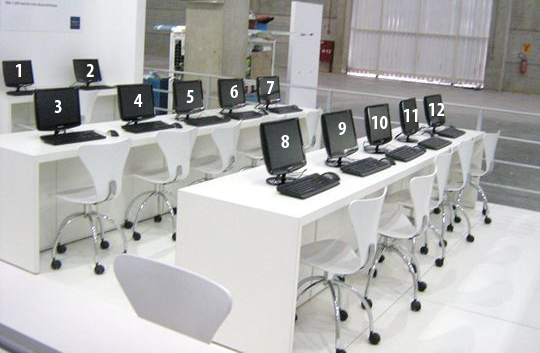
\includegraphics[scale=0.65]{figuras/cap3/sala_computadores.png}
		\caption{\textit{Sala com computadores.}}
		\label{fig:sala_computadores} 
	\end{figure}


    A ARHydra (\textit{Augmented Reality Hydra}) visa amenizar esta tarefa fazendo uso de técnicas de
    Realidade Aumentada. A inserção de informações através de objetos virtuais facilitará na
    identificação dos dispositivos no ambiente inteligente. Os dispositivos serão mapeados através de
    marcadores estrategicamente localizados no dispositivo. De modo que, novas informações a
    respeito dos recursos disponibilizados pelo dispositivo fossem apresentadas para o usuário no
    momento de sua localização.
    
    Esse novo meio de visualização dos recursos proverá uma nova forma de interação entre o
    usuário e o ambiente inteligente. Desta forma, a utilização das facilidades de redirecionamento
    de recursos provida pela Hydra pode ser incrementada com uma visualização, e localização,
    simplificada destes.
    
\subsection{Marcadores na ARHydra}

	Aplicações para a realidade aumentada utilizam marcadores com características próprias, como é
	o caso das aplicações ARToolkit e ARTag. A maior parte dos trabalhos que utilizam esses
	marcadores, associam o código de identificação extraído do marcador a um objeto virtual
	pré-definido. Essa relação causa uma dependência de um mapeamento prévio de todos os objetos 
	virtuais e seus respectivos códigos de identificação, proporcionando uma limitação na interatividade 
	entre novos marcadores.
	
	A ARHydra segue uma estratégia diferente. Utiliza características que favoreçam o reconhecimento e
	a extração de informações através de seus marcadores, sem a necessidade de uma tabela de
	mapeamento. Esse comportamento híbrido proporciona uma interatividade na identificação dos
	marcadores, uma vez que a disponibilidade dos recursos dependem dos dispositivos presentes no
	ambiente.
	 
	A escolha do código QRCode, para identificação dos marcadores, baseia-se na possibilidade de
	inserção de caracteres alfanuméricos, na rápida leitura e na tolerância a erros oferecidas por
	esse código bidimensional. Possibilitando assim, uma forma simplificada para a extração da
	identificação dos dispositivos no ambiente inteligente. 
	
	A figura \ref{fig:arhydra_marcador} exemplifica o marcador utilizado pela ARHydra. Na primeira
	parte da figura é apresentado um marcador utilizado pela aplicação ARToolkit. Em seguida, um
	código QRCode responsável por armazenar alguma informação relevante a respeito do dispositivo. A
	junção dos mesmos formará um marcador constituído de bordas pretas, aos quais delimitam o marcador
	e favorecem uma forma rápida de localização, e o QRCode no centro do marcador, responsável pela
	identificação do marcador.
	
	\begin{figure}[h]
		\centering \includegraphics[scale=0.5]{figuras/cap3/marcador_arHydra.png}
		\caption{\textit{Marcador utilizado na ARHydra.}}
		\label{fig:arhydra_marcador} 
	\end{figure}
	
\subsection{Interação no ambiente}

	Considere o seguinte exemplo de interação da ARHydra com o ambiente. Suponha um 
	\textit{smart space} composto por:
	
	\begin{enumerate}
	  \item Macbook: disponibiliza os recursos de \textit{webcam}, saída de vídeo, \textit{mouse} e
	  teclado;
	  \item \textit{Smartphone} Galaxy SII: disponibiliza os recursos de câmera, mouse e teclado;
	  \item iMac: disponibiliza os recursos de saída de vídeo, \textit{mouse} e teclado.
	\end{enumerate}
	
	No macbook terá uma aplicação utilizando o \textit{uOS} disponibilizando seus recursos através de
	\textit{UpDriver's}, sendo este dispositivo mapeado no ambiente através de um marcador reconhecido
	pela ARHydra. O \textit{smartphone} ficará responsável pela execução da aplicação ARHydra. Por
	fim, a aplicação Hydra será executada no iMac. 
	
	O uso dos marcadores, alinhado com a mobilidade com que o \textit{smartphone} pode interagir com o
	ambiente, faz com que a aplicação ARHydra seja utilizada no \textit{smartphone} do usuário. Essa
	interação possibilita ao usuário uma melhor forma de localização e seleção do recurso disponível.
	
	A figura \ref{fig:apresentacao_arhydra} exemplifica o uso de um marcador para identificar o dispositivo no
	ambiente. Como etapa inicial ilustrada através da figura \ref{fig:visualizacao_qrcode}, há uma
	busca por esse marcador inserido no ambiente, ao qual posteriormente será feito uma tentativa de
	reconhecimento para obtenção da informação contendo os recursos disponibilizados. Com a conclusão
	bem sucedida da etapa anterior, o os recursos serão apresentados ao usuário, conforme ilustrado na
	figura \ref{fig:visualizacao_obj}. Essa exibição é feita utilizando técnicas da realidade
	aumentada. Por fim, a aplicação ARHydra possibilita ao usuário escolher qual recurso deseja que
	seja redirecionado para a Hydra.
	
	\begin{figure}[htb]
		\centering
			\subfloat[Visualização do marcador]{
				\label{fig:visualizacao_qrcode}
				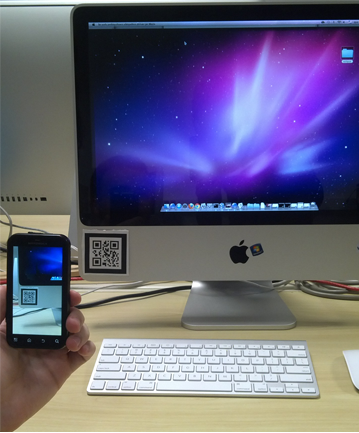
\includegraphics[width=0.45\textwidth]{figuras/cap3/visao_mac.png}
			}
			\subfloat[Visualização do objeto virtual]{
				\label{fig:visualizacao_obj}
				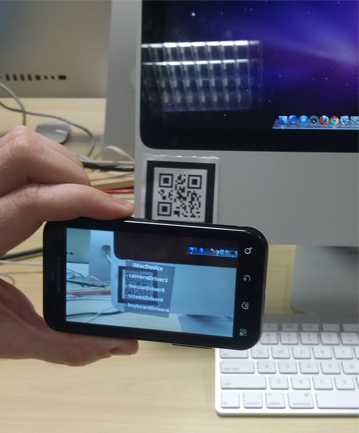
\includegraphics[width=0.45\textwidth]{figuras/cap3/visao_qrcode.png}
			}
		
		\caption{\textit{(a) Exemplo da visão do usuário para a busca do marcador do dispositivo. (b)
		Exemplo da visualização do objeto virtual apresentando os recursos disponíveis}}
		\label{fig:apresentacao_arhydra} 
	\end{figure}
	
	
	A interação da ARHydra no ambiente inteligente segue os passos observados na figura~\ref{fig:arhydra_interacao}:

	\begin{figure}[h] 
		\centering 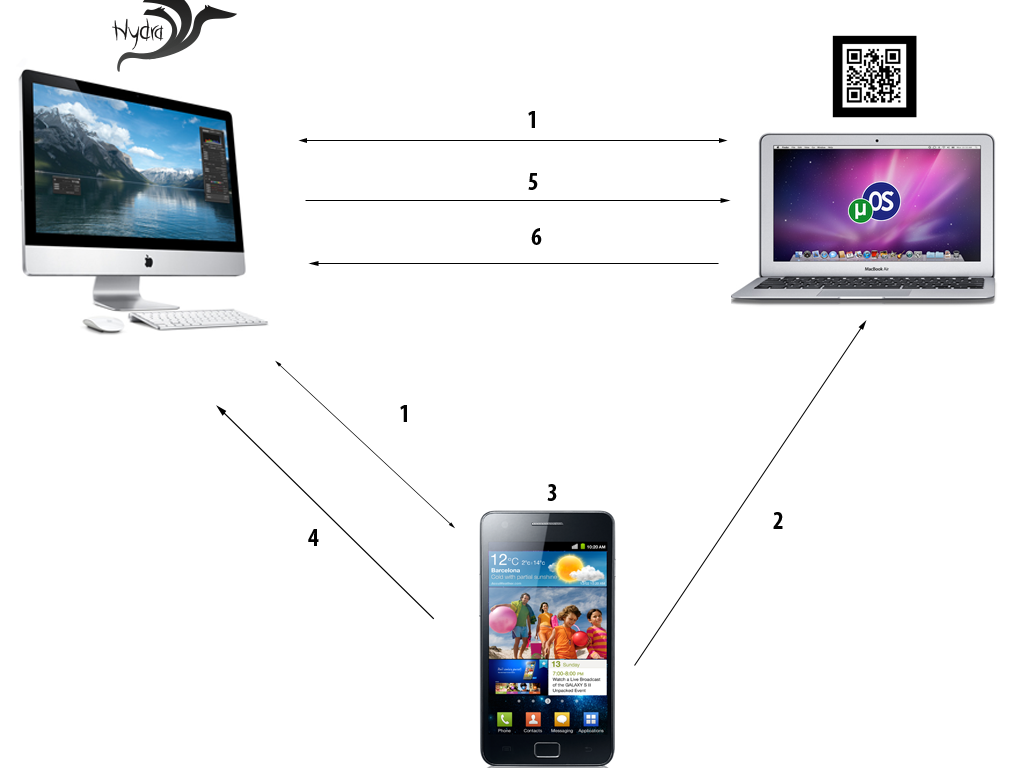
\includegraphics[scale=0.45]{figuras/cap3/integracao_arhydra.png}
		\caption{\textit{Integração Hydra com o ambiente.}}
		\label{fig:arhydra_interacao} 
	\end{figure}
	
	\begin{enumerate}
	  \item A Hydra implementa o mecanismo de descoberta de novos dispositivos e os registra os
	  dispositivos encontrados em sua base de dados;
	  
	  \item A ARHydra procura o marcador identificador do Macbook;
	  
	  \item Faz a reconhecimento e decodificação do marcador encontrado, busca os recursos disponíveis
	  do dispositivo e apresenta esses recursos na tela do \textit{smartphone} com os recursos
	  providos pela realidade aumentada, possibilitando ao usuário selecionar um recurso disponível.
	  
	  \item Caso o usuário selecione um recurso, a ARHydra faz uma requisição à Hydra para que
	  redirecione o recurso selecionado do Macbook para o uso na Hydra.
	  
	  \item A Hydra recebe a solicitação vinda do \textit{smartphone}, solicita o registro do
	  recurso selecionado para a aplicação do \textit{uOS} executada no Macbook.
	  
	  \item A partir desse momento, o recurso do Macbook selecionado pela ARHydra será redirecionado
	  para o iMac.
	\end{enumerate}

	Com isso, a aplicação ARHydra complementa a interação do usuário com a Hydra, auxiliando na
	identificação visual dos dispositivos e no redirecionamento dos recursos disponíveis. 
 	

	


	\chapter{Implementação e testes}
\label{cap:implementacao_testes}

%\epigraph{`` Modernizar não é sofisticar. Modernizar é simplificar.''}{Joelmir Beting}


	A ARHydra tem por objetivo prover uma interface de interação aprimorada à Hydra, de modo que o
	usuário tenha uma maior transparência e facilidade na seleção dos recursos do ambiente. No capítulo
	anterior foi detalhado o seu uso, já neste serão apresentados os aspectos relativos a sua
	implementação. Neste sentido será enfatizada a sua arquitetura e os testes realizados.
	
	A aplicação foi desenvolvida para ser utilizada em \textit{smartphones} dotados de tela sensível ao toque e câmera.
	Tais dispositivos são adequados para a realidade aumentada devido a mobilidade, além disso permite 
	que o usuário interaja com o ambiente e a informação de forma direta (Visão Direta). Como
	plataforma foi utilizada o sistema Android que faz uso da máquina virtual Dalvik. Esta escolha
	permitiu o uso do~\textit{middleware uOS}, desenvolvido em Java, sem grandes complicações.

 	A figura \ref{fig:interacao_modulos} apresenta como os quatro módulos da aplicação interagem entre
 	si. O fluxo tem início com a obtenção da imagem capturada pela câmera do celular. Este é repassado
 	ao Módulo de Reconhecimento (seção~\ref{sec:modulo_reconhecimento}) onde são encontrados os
 	marcadores presentes na imagem sendo exibida. Identificado um marcador é então calculado seu
 	centro, bem como a sua orientação.
 	
	Conhecendo a posição do marcador na imagem cabe ao Módulo de Decodificação
	(seção~\ref{sec:modulo_decodificacao}) extrair a informação presente. Esta consiste de um código
	identificador do dispositivo representado, sendo utilizado na localização dos recursos
	disponíveis.
	
	Conhecendo as informações sobre o dispositivo, cabe ao Módulo de Apresentação
	(seção~\ref{sec:modulo_apresentacao}) desenhar o objeto virtual na tela. As informações que compõe
	esse objeto são obtidas a partir da integração entre a Hydra e a ARHydra, tarefa esta sob
	responsabilidade do Módulo de Integração (seção~\ref{sec:modulo_integracao}). No objeto virtual são
	exibidas as informações que auxiliem o usuário na sua escolha, sendo estas composta pelo nome do
	dispositivo e os recursos por ele disponibilizados. Por fim, o Módulo de Integração possibilita ao
	usuário o redirecionamento ou a liberação de um recurso.
	
	Tanto o Módulo de Reconhecimento quanto o Módulo de Decodificação possuem suas próprias linhas de
	execução, ocasionando uma interação assíncrona entre esses módulos. Por causa desse tipo de
	interação, a comunicação entre esses módulos é feita através de eventos, isso propicia que seja
	mantida a interação junto ao usuário enquanto o processamento é realizado em segundo plano.
	
	\begin{figure}[htb]
		\centering 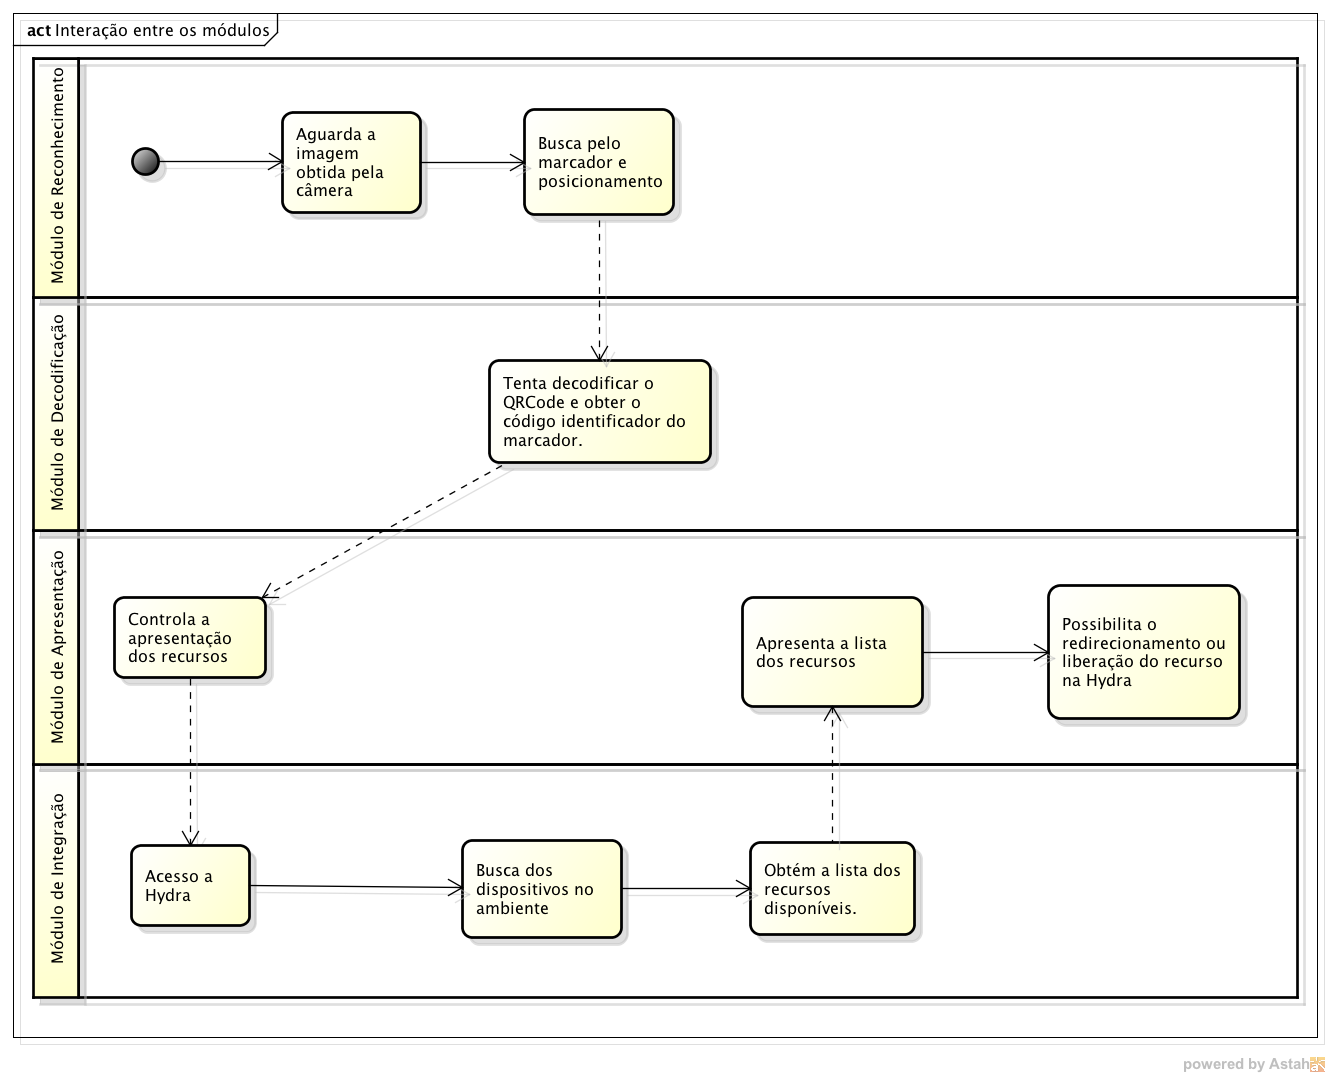
\includegraphics[scale=0.45]{figuras/cap4/interacao_modulos.png}
		\caption{\textit{Interação entre os módulos.}}
		\label{fig:interacao_modulos} 
	\end{figure}

	\section{Módulo de Reconhecimento}
\label{sec:modulo_reconhecimento}

	
	Neste módulo é realizada o reconhecimento dos marcadores bem como a obtenção de sua posição na
	imagem do ambiente. Este é notificado a cada imagem nova capturada pela câmera do dispositivo e de
	posse desta sua linha de execução inicia os passos apresentados na figura \ref{fig:processo_detect} e
	conforme descrito a seguir:
	
	\begin{figure}[h]
		\centering 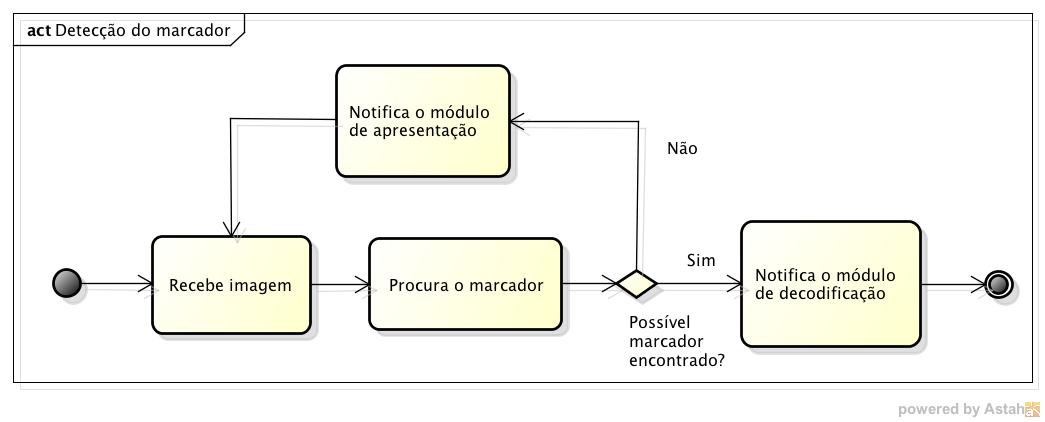
\includegraphics[scale=0.55]{figuras/cap4/processo_deteccao.png}
		\caption{\textit{Processos do Módulo de Reconhecimento.}}
		\label{fig:processo_detect} 
	\end{figure}
	
	\begin{enumerate}

	  \item A imagem obtida é convertida para escala de cinza com o intuito de se obter uma 
	  	homogeneidade da coloração dos \textit{pixels}. Desta forma a detecção de padrões ocorre de forma 
	  	facilitada.
	  
	  \item Utilizando a biblioteca OpenCV é realizada a correção de perspectiva da imagem, já que 
	  	o ângulo observado é distinto da figura esperada (vista frontal). Através da mesma biblioteca 
	  	é realizada a detecção de contornos, com base na borda negra do marcador, e determinação dos 
	  	quatro pontos que a delimitam.
	  	
	  \item Estima-se o posicionamento do marcador baseado nos quatro pontos não lineares
	  		identificados no passo anterior. Nesse procedimento também é obtido o ponto central da imagem,
	  		responsável pelo posicionamento correto do objeto virtual a ser sobreposto ao marcador.
	  
	  \item Para a obtenção da orientação do marcador foi utilizado o sensor de orientação disponível pelo
	  		\textit{smartphone}. A partir dessas informações é possível estimar o ângulo correto de visão
	  		do \textit{smartphone}, posicionando o objeto virtual corretamente.
	  		
	\end{enumerate} 
	
	Caso os quatro passos sejam executados com sucesso, tanto o marcador quanto sua posição seja obtida 
	com sucesso, estas informações são repassadas ao Módulo de Decodificação para que se prossiga com o fluxo 
	normal da aplicação. Caso contrário, é feita uma contagem para analisar se o marcador ainda está sendo 
	capturado pela câmera do celular. Se o processo em andamento atingiu a quantidade máxima de tentativas 
	consecutivas sem sucesso, o Módulo de Apresentação é notificado a respeito que nenhum marcador foi encontrado na 
	imagem, desta forma é possível atualizar a visão do usuário. Independente de ter ocorrido um reconhecimento, 
	o módulo voltará a aguardar	uma nova imagem para que um novo procedimento seja feito.
	
	Apesar da plataforma Android aceitar aplicações que sejam desenvolvidas utilizando a linguagem Java é
	possível combinar aplicações Java com aplicações e bibliotecas desenvolvidas em C/C++. Essa
	integração ocorre através do JNI (\textit{Java Native Interface}) suportada pelo 
	NDK \textit{(Native Development Kit)}. Tirando proveito deste suporte, este módulo integra-se com
	a solução elaborada para o reconhecimento através de uma conexão utilizando o JNI, devido ao fato
	do processo de reconhecimento utilizar a biblioteca \textit{OpenCV}, implementada utilizando a
	linguagem C.

	\section{Módulo de Decodificação}
\label{sec:modulo_decodificacao}

	Conhecendo a imagem do marcador encontrado cabe a este módulo extrair a informação representada por 
	ele. Para isto são utilizados marcadores QRCode ao qual representa o nome do dispositivo. Desta forma é 
	possível encontrar os recursos (\textit{drivers}) por este disponibilizados. Assim como o Módulo de Reconhecimento, 
	este módulo consiste em uma linha de execução própria e seu fluxo de execução ocorre conforme representado 
	na Figura \ref{fig:processo_decode} e descrito a seguir.
	
	\begin{figure}[htb]
		\centering 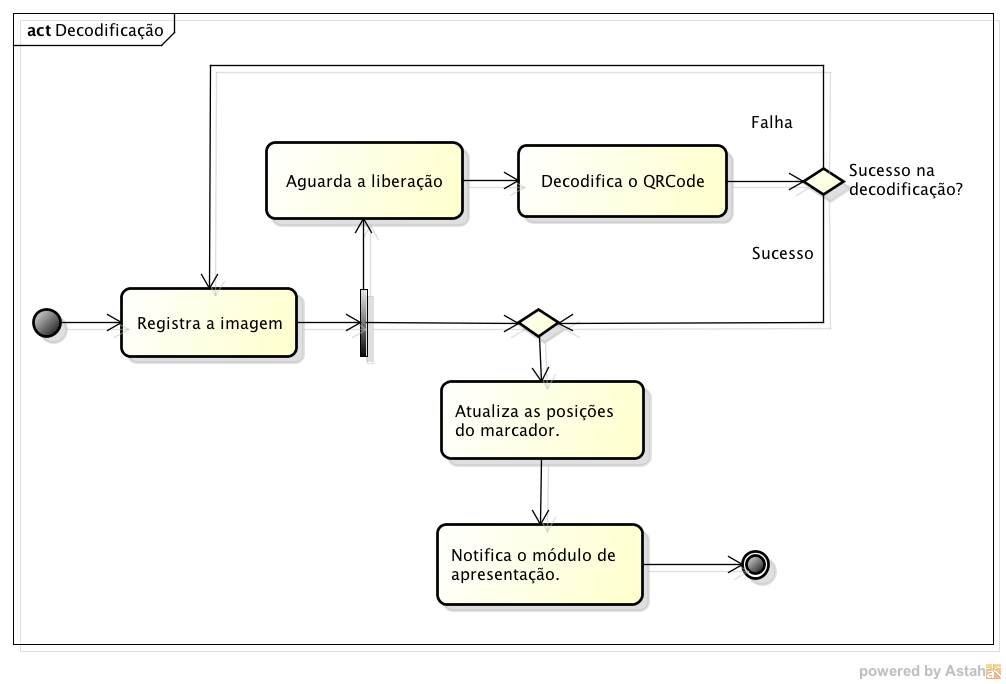
\includegraphics[scale=0.6]{figuras/cap4/processo_decodificacao.png}
		\caption{\textit{Processos do Módulo de Decodificação.}}
		\label{fig:processo_decode} 
	\end{figure}
	
	O Módulo de Decodificação é criado junto com o módulo de Reconhecimento, no entanto sua execução é 
	iniciada após o recebimento de algum marcador encontrado pelo Módulo de Reconhecimento. O marcador 
	recebido é registrado para que seja feito a atualização das informações a respeito da imagem recebida.
	Com o registro efetuado com sucesso é dado início ao processo de decodificação do marcador recebido. 
	Pelo fato do processo de reconhecimento ser mais rápido quando comparado ao processo de decodificação
	fez-se necessário a criação de um controle para que fosse garantido uma correta sincronização na 
	decodificação dos marcadores. Por essa razão, ocorrerá o descarte de qualquer marcador recebido enquanto 
	houver um processo de decodificação em execução. 
	
	Foi criado um Gerenciador com o propósito de centralizar todas as informações necessárias, de classes e 
	procedimentos, envolvidas no processo de decodificação. Ele age como uma interface entre o Módulo de 
	Decodificação e as aplicações responsáveis pela decodificação. A aplicação ZBar~\cite{zbar} foi utilizada 
	como ferramenta suporte ao processo de decodificação. Esta ferramenta é implementada utilizando a linguagem C. 
	Por essa razão a integração entre a aplicação ZBar com a ARHydra ocorre através do JNI. 
	
	As posições do marcador são atualizadas após o processo de decodificação ser finalizado com sucesso, ou seja, 
	houve êxito na obtenção do código de identificação do marcador analisado. Essa mesma etapa correspondente a  
	atualização das posições é feita quando um marcador é recebido do Módulo de Reconhecimento. Essa tarefa tem 
	um comportamento assíncrono devido o processo de decodificação ser um processo oneroso quando comparado dos 
	demais procedimentos separadamente. Por essa razão, enquanto houver um processo de decodificação em execução, as 
	posições referentes ao objeto virtual apresentado ao usuário são atualizadas com as informações recebidas
	pelos marcadores enviadas do Módulo de Reconhecimento. Após a atualização, essas informações são repassadas 
	ao Módulo de Apresentação para que as informações correspondentes ao marcador sejam atualizadas e apresentadas 
	ao usuário.
	
	Por outro lado, caso o processo de decodificação não consiga obter o código identificador correspondente ao 
	marcador analisado, o Módulo de Decodificação enviará uma notificação para o Módulo de Apresentando informando 
	a não possibilidade de detecção do código identificador do marcador, desta forma é possível atualizar a visão
	do usuário. Após a conclusão dessa notificação, o Módulo de Decodificará aguardará o recebimento da próxima 
	imagem enviada pelo Módulo de Reconhecimento, reinicializando todos os procedimentos até aqui apresentados 
	para este módulo.
	
	
	\section{Módulo de Integração} 
\label{sec:modulo_integracao}

	Na composição do objeto virtual é necessário reunir informações relevantes sobre a disponibilidade dos 
	recursos provido pelo dispositivo escolhido. O Módulo de Integração é responsável pela integração da 
	ARHydra com a Hydra com o propósito de criar um canal de comunicação entre essas duas aplicações. Esta 
	integração é feita através de \textit{drivers} de comunicação, conforme	estabelecido pela DSOA. 
	
	Quando um recurso apresentado pelo dispositivo é selecionado faz-se necessário informar a Hydra	qual 
	recurso fora escolhido. Esse canal externo de comunicação entre as aplicações não é fornecida pelo 
	\textit{uOS} de forma nativa. Por essa razão, a arquitetura inicial da Hydra 
	não implementou nenhuma forma para o recebimento de requisições externas. Permite apenas a interação 
	via terminal de aplicação, ou seja, sem acesso por outras aplicações. Desta forma, para o usuário 
	redirecionar algum recurso, ele terá que ir até o dispositivo executando a Hydra e prover o 
	redirecionamento de forma manual. Para realizar essa comunicação foi desenvolvido um~\textit{driver} 
	na Hydra que possibilitasse o recebimento de requisições externas. O envio das requisições, bem como
	o recebimento das respostas realizadas pelas mesmas, decorrentes dessa comunicação, ocorre através do 
	Módulo de Integração.  

	Para economizar recursos do \textit{smartphone}, a obtenção da informação de quais dispositivos
	estão disponíveis dentro do ambiente inteligente fica sob responsabilidade da Hydra, ao qual implementará
	mecanismos para identificação dos dispositivos no ambiente através da utilização de radares. A ARHydra 
	possui um mecanismo de agendamento para que essa informação seja atualizada. Com a periodicidade de 60 segundos, 
	o Módulo de Integração envia informações para a Hydra requisitando quais são os dispositivos que estão 
	ativos dentro do ambiente.
	
	\section{Módulo de Apresentação}
\label{sec:modulo_apresentacao}

	Após o marcador ser reconhecido e identificado, o Módulo de Apresentação fica responsável por
	apresentar ao usuário todos os recursos disponíveis do dispositivo selecionado. São aceitos os
	mesmos recursos compatíveis com a Hydra: câmera, \textit{mouse}, teclado ou tela. Os recursos são
	visualizados através de um objeto virtual, ao qual é apresentado na tela. Este é representado
	através de um retângulo onde é exibido o nome do dispositivo e os recursos por ele
	disponibilizados. Na figura \ref{fig:objeto_virtual}, podemos observar um caso onde temos o 
	dispositivo iMacDevice que disponibiliza os seus recursos de câmera,~\textit{mouse}, tela e teclado.

	
	\begin{figure}[htb]
		\centering 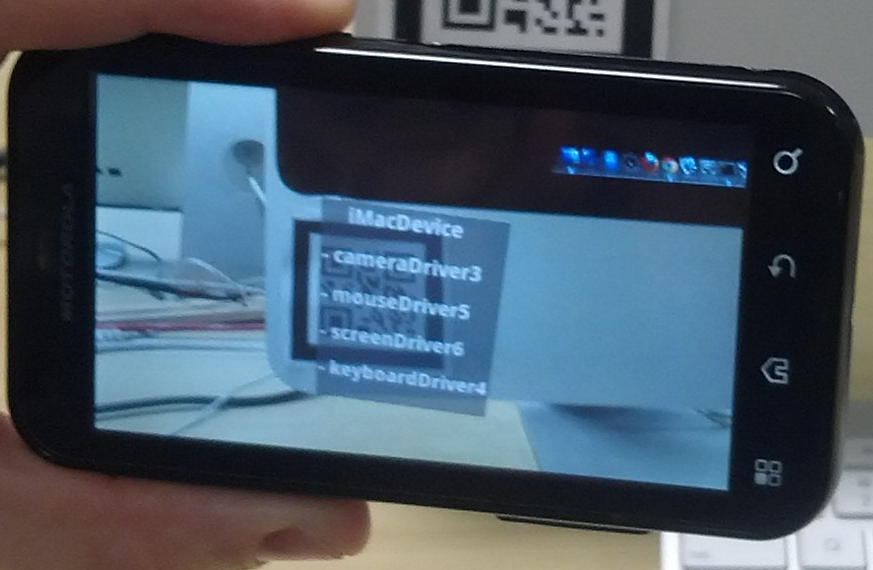
\includegraphics[scale=0.3]{figuras/cap4/objeto_virtual.png}
		\caption{\textit{Objeto virtual.}}
		\label{fig:objeto_virtual} 
	\end{figure}
	
	Para interagir com o dispositivo basta ao usuário tocar a tela sobre o objeto que o representa.
	Desta forma é exibida uma nova tela onde é possível controlar o uso dos recursos do dispositivo.
	Possibilitando ao usuário selecionar o redirecionamento ou liberação conforme desejado. A 
	figura~\ref{fig:listagem_recursos} mostra o detalhamento dos recursos disponíveis ao usuário no 
	dispositivo. Os recursos de teclado e \textit{mouse} já estão sendo redirecionados para a Hydra, 
	enquanto os demais estão disponíveis para serem utilizados pela mesma.
	
	
	\begin{figure}[htb]
		\centering 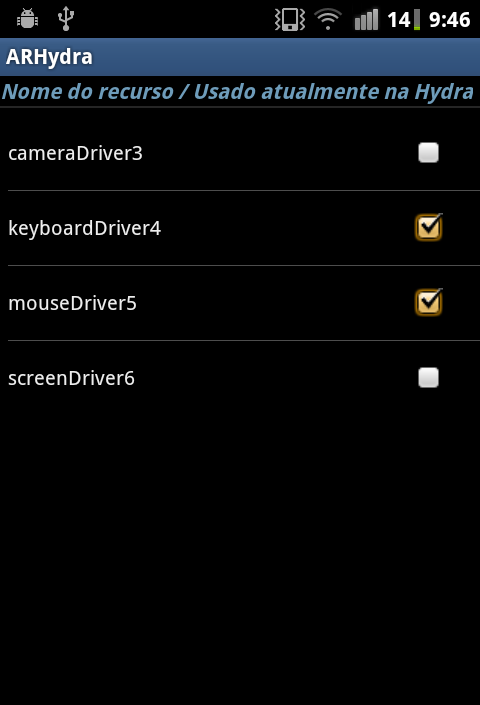
\includegraphics[scale=0.35]{figuras/cap4/listagem_recursos.png}
		\caption{\textit{Listagem dos recursos.}}
		\label{fig:listagem_recursos} 
	\end{figure}
	
	O \textit{framework} DroidAR \cite{droidar} foi utilizado para facilitar a renderização dos objetos 
	na tela. Para o gerenciamento desses objetos virtuais fez-se necessário a criação de uma classe 
	responsável pela criação, reposicionamento e deleção desses objetos. Essa classe recebe informações
	dos Módulos de Reconhecimento e Decodificação para determinar a ação a ser executada. A interação
	desse controle com os demais módulos é apresentado na figura~\ref{fig:condicoes_objeto}.

	\begin{figure}[htb]
		\centering 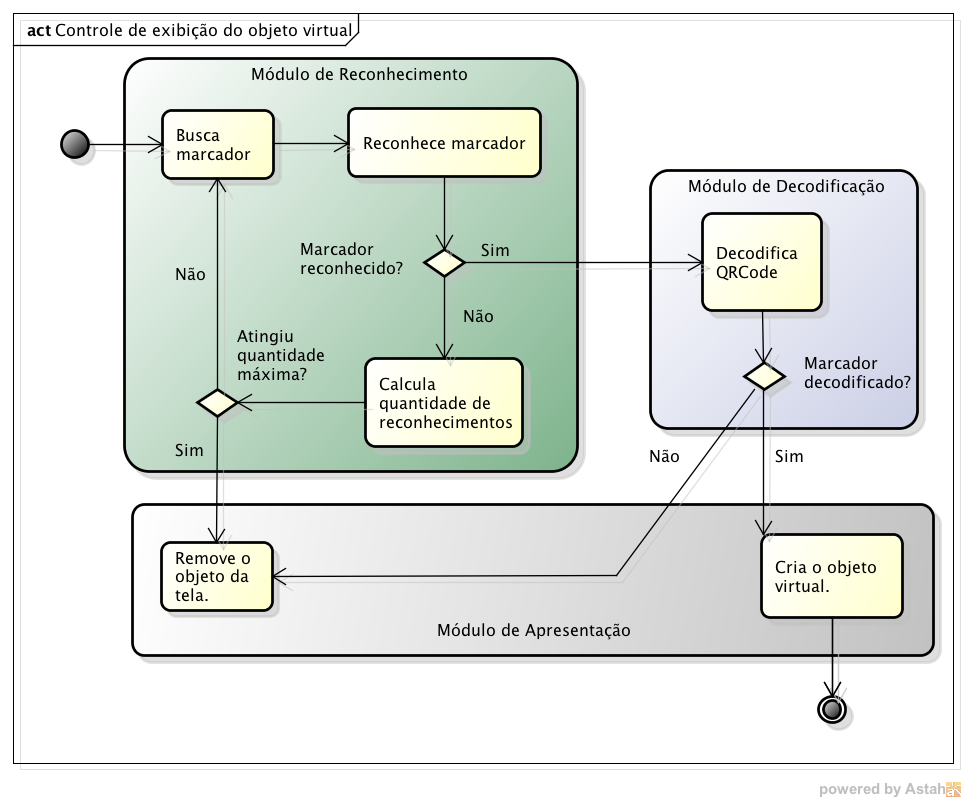
\includegraphics[scale=0.55]{figuras/cap4/condicoes_objeto.png}
		\caption{\textit{Condições para visualização do objeto virtual.}}
		\label{fig:condicoes_objeto} 
	\end{figure}

	Desta maneira, o controle de exibição dos objetos virtuais possibilita uma correta visualização
	dos recursos disponíveis pelos dispositivos. De modo que somente os recursos de um dispositivo
	sejam apresentados por vez.
	

	\section{Hydra \textit{Driver}}
\label{sec:hydradriver}

	A aplicação Hydra foi concebida para ter seu controle realizado pelo usuário diretamente na máquina de 
	onde os recursos seriam direcionados. Desta forma, não seria possível que outros dispositivos solicitassem 
	que um novo redirecionamento seja realizado. Para superar esta limitação foi desenvolvido um~\textit{driver} 
	denominado~\textit{HydraDriver} que disponibiliza as opções de interação da Hydra no~\textit{Smart Space}.
	
	Este recurso visa replicar as mesmas capacidades disponíveis na interface gráfica da aplicação original 
	sendo composto por um conjunto de três serviços síncronos:
	
	\begin{enumerate}
	  \item \textbf{Redirecionamento do recurso:} Com este serviço é possível redirecionar um recurso da 
	  	máquina para um disponível em outro dispositivo.
	  
	  \item \textbf{Liberação do recurso:} Informado o recurso desejado e o dispositivo a ele relacionado, 
	  	é finalizado o redirecionamento existente entre eles.
	  
	  \item \textbf{Uso do recurso:} Retorna as informações acerca do recurso local. Nestas informações 
	  	é possível observar se ele está em uso no momento e para qual dispositivo está sendo redirecionado.
	  
	\end{enumerate}	
	

	\section{Testes}
	
	A operação da aplicação ARHydra está diretamente relacionada ao tempo que esta necessita para levar a informação ao 
	seu usuário. Com o objetivo de medir este tempo foram realizados testes onde se variou a distância do marcador 
	bem como o equipamento utilizado. Os dados foram analisados com relação a execução completa dos três componentes 
	envolvidos na operação (reconhecimento, decodificação e apresentação). Estes testes foram realizados no ambiente do 
	LAICO (LAboratorio de Sistemas Integrados e COncorrentes), situado no Departamento de Ciências da Computação da 
	Universidade de Brasília. Foram utilizados dois~\textit{smartphones} distintos, um Motorola Defy e um 
	Sansung Galaxy SIII, de forma a avaliar a influência da qualidade da câmera e do processamento durante o uso. O Motorola 
	Defy possui as seguintes especificações: processador Cortex-A8 de 800 MHz, 512 MB de memória RAM, resolução de tela 
	de 480 x 854~\textit{pixels}, GPU (\textit{Graphics Processing Unit}) PowerVR SGX530 e câmera com resolução de 5MP. 
	O Sistema Operacional testado nesse dispositivo foi o Android 2.3.7 com~\textit{firmware} CyanogenMod 7.2. Já o 
	\textit{smartphone} Samsung Galaxy SIII possui processador Quad-core 1.4 GHz Cortex-A9, 1GB de memória RAM, 
	resolução da tela de 720 x 1280~\textit{pixels}, GPU Mali-400MP, câmera com resolução de 8MP e sistema operacional 
	Android 4.0.4.

\subsection{Reconhecimento dos marcadores}
	
	Foram executados conjuntos de testes com o objetivo de mensurar o tempo gasto no processo de
	reconhecimento do marcador proposto. O tempo de reconhecimento é composto pela soma dos tempos gasto
	na identificação das bordas do marcador, do processo de decodificação do QRCode, da obtenção dos
	dados (via integração com a Hydra) referentes ao marcador selecionado e da apresentação dos
	recursos ao usuário. Deste modo, foram propostos testes que realizassem as seguintes medições:
		
	\begin{enumerate}
	  \item \textbf{Medição do tempo do primeiro reconhecimento:} Tempo com que o
	  		marcador é reconhecido pela primeira vez após a aplicação ARHydra ser inicializada;
	  
	  \item \textbf{Medição do tempo de recorrência:} Tempo com que a aplicação gasta para
	  		reconhecer um marcador de forma recorrente, conforme a câmera é movimentada sem que a mesma
	  		perca a visualização do marcador;
	  
	  \item \textbf{Medição do tempo de reconhecimento após o marcador não estar mais no campo de visão da
	  		câmera do \textit{smartphone}:} Tempo médio necessário para que a aplicação
	  		reconheça um novo marcador após o usuário perder o campo de visão do marcador
	  		no~\textit{smartphone}.
	  		
	  \item \textbf{Taxa de erros:} Este valor representa o percentual das ocorrências com que a
			aplicação ARHydra deixou de identificar o marcador quando este estava sendo capturado pela câmera
			do~\textit{smartphone}.
	   
	   \item \textbf{Taxa de não decodificação:} Este valor representa a porcentagem média de falha nas decodificações 
	   		do QRCode inseridos no marcador. As ocorrências nesta taxa são contabilizadas quando um marcador é reconhecido
	   		porém não é feita a decodificação do QRCode pelo Módulo de Decodificação. Esse valor varia de acordo 
	   		com a aplicação responsável pela decodificação, o nível de tolerância a falhas utilizada no QRCode, a 
	   		qualidade da obtenção das imagens pelo dispositivo e a distância entre o marcador e o~\textit{smartphone}. 
	
	\end{enumerate}
	
	A aplicação ARHydra oferece suporte, presente no Módulo de Decodificação, para a utilização de diversos 
	aplicativos ao qual disponibilizem o recurso de decodificação de QRCode's. Através desse suporte foram 
	realizados testes que permitiram estabelecer um comparativo de desempenho entre essas diversas aplicações 
	utilizadas. A fim de obter esse comparativo, as aplicações ZBar~\cite{zbar} e ZXing~\cite{zxing} foram	
	utilizadas nos referidos testes.
	
	Uma outra informação importante a ser definida refere-se ao estabelecimento de uma distância máxima
	para o reconhecimento destes marcadores. Este valor pode variar de acordo com a aplicação
	utilizada no processo de decodificação, considerando as limitações envolvidas no recolhimento das
	informações necessárias para a decodificação mesmo quando os QRCode's apresentarem níveis de
	tolerância a falhas. Desta maneira, para o estabelecimento desse valor, os testes propostos foram
	executados para diferentes distâncias.
	
	As taxas de erros e de não decodificação estão diretamente relacionadas a qualidade da imagem obtida. No entanto,
	esta qualidade não diz respeito somente a resolução da câmera utilizada, outros fatores podem influenciar no
	reconhecimento do marcador. Dentre estes pode-se citar a qualidade das lentes e o algoritmo utilizado na compressão 
	das imagens, possibilitando que seja obtido resultados diferentes para cenários semelhantes, quando estes 
	resultados são coletados utilizando dispositivos dotados de diferentes câmeras. Um outro ponto importante 
	para se garantir esta qualidade está no controle de luminosidade implementado pelas câmeras. Para minimizar esses 
	problemas apresentados é possível ser implementado etapas de pré-processamento da imagem para melhorar a qualidade
	dessa imagem obtida.
	
\subsubsection{Especificações do Marcador}

	O marcador foi construído baseando nas especificações apresentadas pelo QRCode
	(seção~\ref{sec:simbolos_bidimensionais}) e nas dimensões necessárias voltadas para o módulo de
	reconhecimento validar o marcador. Também deve ser considerado a inserção desses marcadores no ambiente de forma menos
	intrusiva possível, mas que suas caraterísticas possibilitem seu reconhecimento.
	
	A Figura~\ref{fig:dimensoes_marcador} apresenta as dimensões adotadas na construção desses
	marcadores. O QRCode é envolvido por uma moldura, com bordas no valor experimental de 0,8 centímetros, 
	para que o módulo de reconhecimento consiga validar e estabelecer as informações de
	posicionamento referentes ao marcador e o módulo de decodificação realize com sucesso a decodificação
	do QRCode.
	
	\begin{figure}[htb]
		\centering 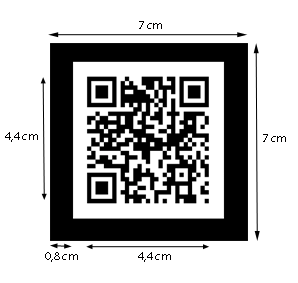
\includegraphics[scale=0.8]{figuras/cap4/dimensoes_marcador.png}
		\caption{\textit{Dimensões do marcador.}}
		\label{fig:dimensoes_marcador} 
	\end{figure}
	
\subsection{Resultados}
\label{sec:resultados}

	Os conjuntos de testes foram executados a uma distância inicial de 50
	centímetros, referente a distância entre o marcador e a aplicação ARHydra executada
	no~\textit{smartphone}, sendo esta aumentada gradativamente em 10 centímetros até atingir o valor 
	de 1 metro. Foram executados os seguintes testes:
	
	\begin{itemize}
	  \item Desempenho e qualidade da obtenção da imagem: Neste teste foi utilizado dois
	  		~\textit{smartphones} com o propósito de estabelecer a diferença de desempenho da aplicação
	  		ARHydra, bem como apresentar o comparativo entre taxas de reconhecimento e não decodificação 
	  		do QRCode para cada~\textit{smartphone} utilizado.
	  
	  \item Suporte a diversas aplicações de decodificação do QRCode: Neste teste foi validado o suporte 
	  		oferecido pela ARHydra para a utilização de diversos aplicativos cujo propósito seja a 
	  		decodificação de QRCodes.
	  		
	  \item Influência da tolerância a falhas do QRCode: Este permite medir a influência dos níveis de 
	  		tolerância a falhas aplicados ao QRCode e sua relação com a taxa de não decodificação.
	  			  
	\end{itemize}

\subsubsection{Teste de desempenho e qualidade na obtenção da imagem}
\label{sec:testesDesempenho}

 
	Um dos objetivos para este teste é comparar o desempenho da aplicação ARHydra utilizada nos dispositivos mencionados 
	anteriormente, com o propósito de  mensurar a diferença nos tempos de reconhecimento do marcador, sendo esta 
	influenciada diretamente pela capacidade de processamento, processador e~\textit{GPU}, de cada dispositivo. O outro 
	objetivo consiste em analisar a influência da qualidade da imagem obtida pela câmera, destes dispositivos, estabelecendo 
	um comparativo entre as taxas de erro e não decodificação.
	
	Para a execução do teste foram realizadas vinte medições para a primeira aparição, duzentas medições para as recorrências 
	e cinquenta medições para o reconhecimento ao perder o marcador. Os resultados dessas medições são apresentados nos 
	gráficos das Figuras~\ref{fig:testeCompDesempenho} e \ref{fig:testeCompTaxas}.
	
	\begin{figure}[htb] 
		\centering 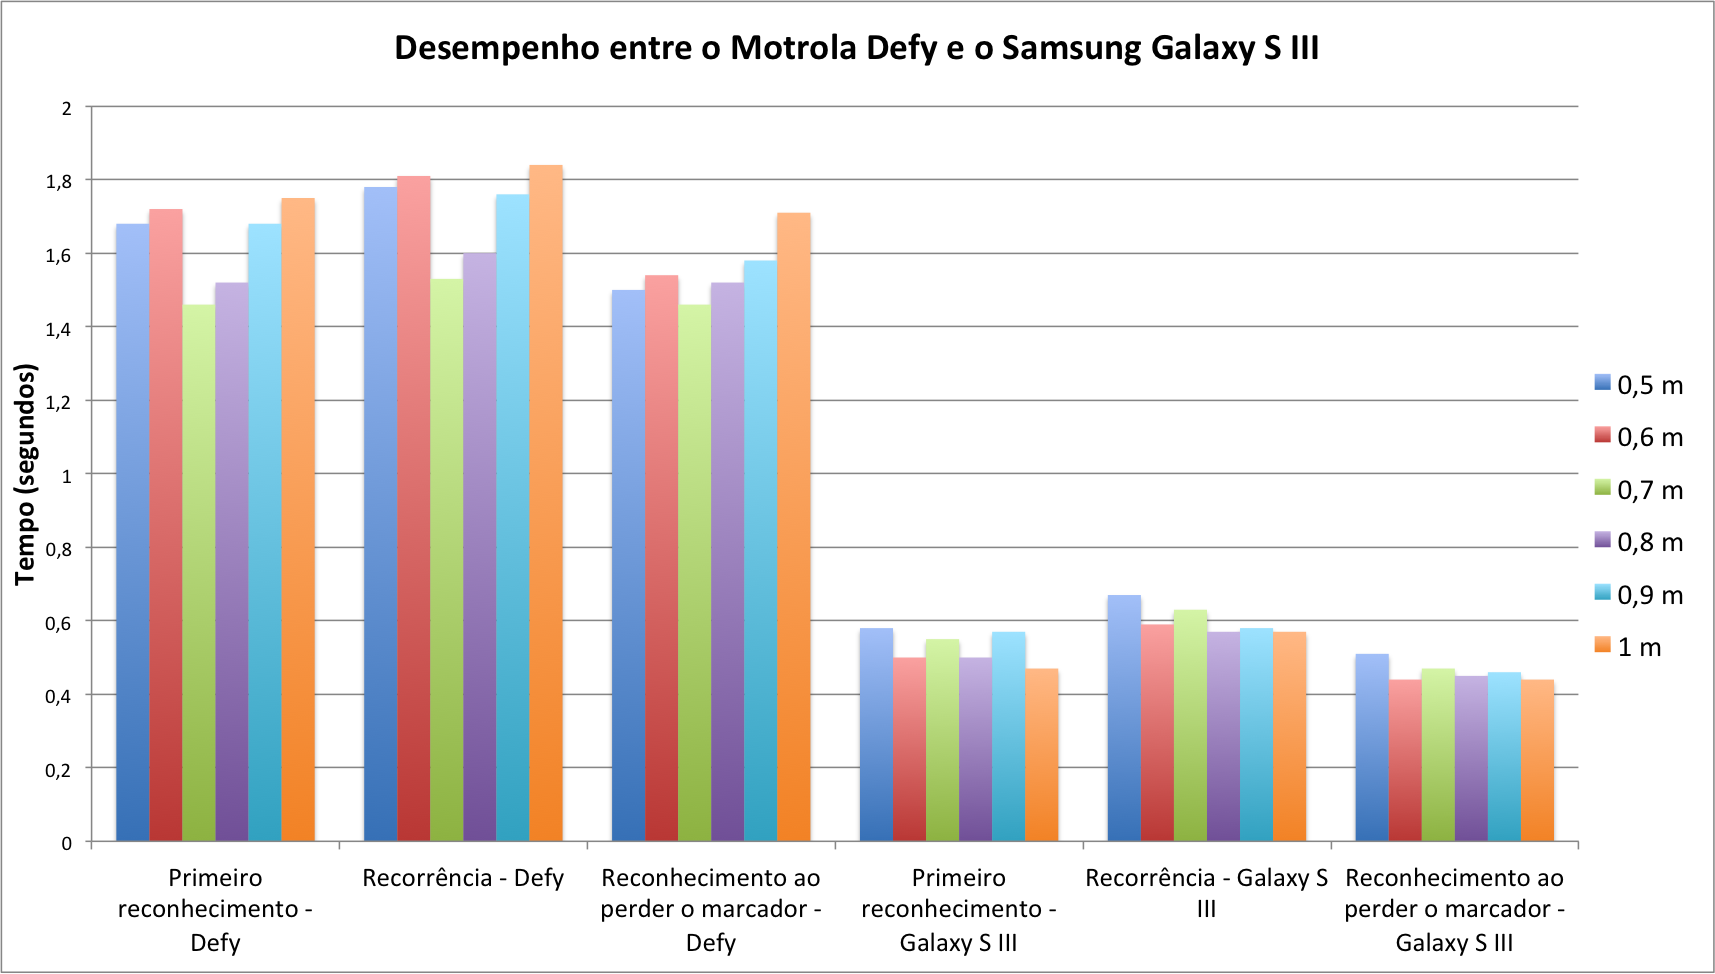
\includegraphics[scale=0.55]{figuras/cap4/grafico_desempenho.png}
		\caption{\textit{Comparativo de desempenho da aplicação ARHydra entre os dispositivos Motorola Defy e 
							Samsung Galaxy SIII.}}
		\label{fig:testeCompDesempenho} 
	\end{figure}
	
	
	A Figura \ref{fig:testeCompDesempenho} apresenta o resultado que mede o desempenho dos dispositivos. Ela mostra que o 
	dispositivo Galaxy SIII obteve melhor desempenho, sendo mais rápido no reconhecimento dos marcadores, devido a diferença 
	na capacidade de processamento, processador e~\textit{GPU}, presente no processador do Galaxy SIII. Desta forma, 
	quanto maior for a capacidade de processamento do dispositivo menor será o tempo gasto pela aplicação ARHydra reconhecer
	os marcadores.   
	
	Os tempos obtidos no primeiro reconhecimento foram inferiores quando comparados ao tempo gasto na recorrência, em ambos 
	os dispositivos, por causa da baixa quantidade de imagens a serem processadas ou descartadas pelos módulos de 
	reconhecimento,	decodificação e apresentação após a captura das imagens ser inicializada. Adicionalmente, a 
	aplicação ARHydra não apresenta um mecanismo de histórico de reconhecimentos ocasionando com que cada 
	reconhecimento concluído com sucesso seja considerado um novo reconhecimento, onerando assim o tempo de recorrência. 
	
	\begin{figure}[htb] 
		\centering 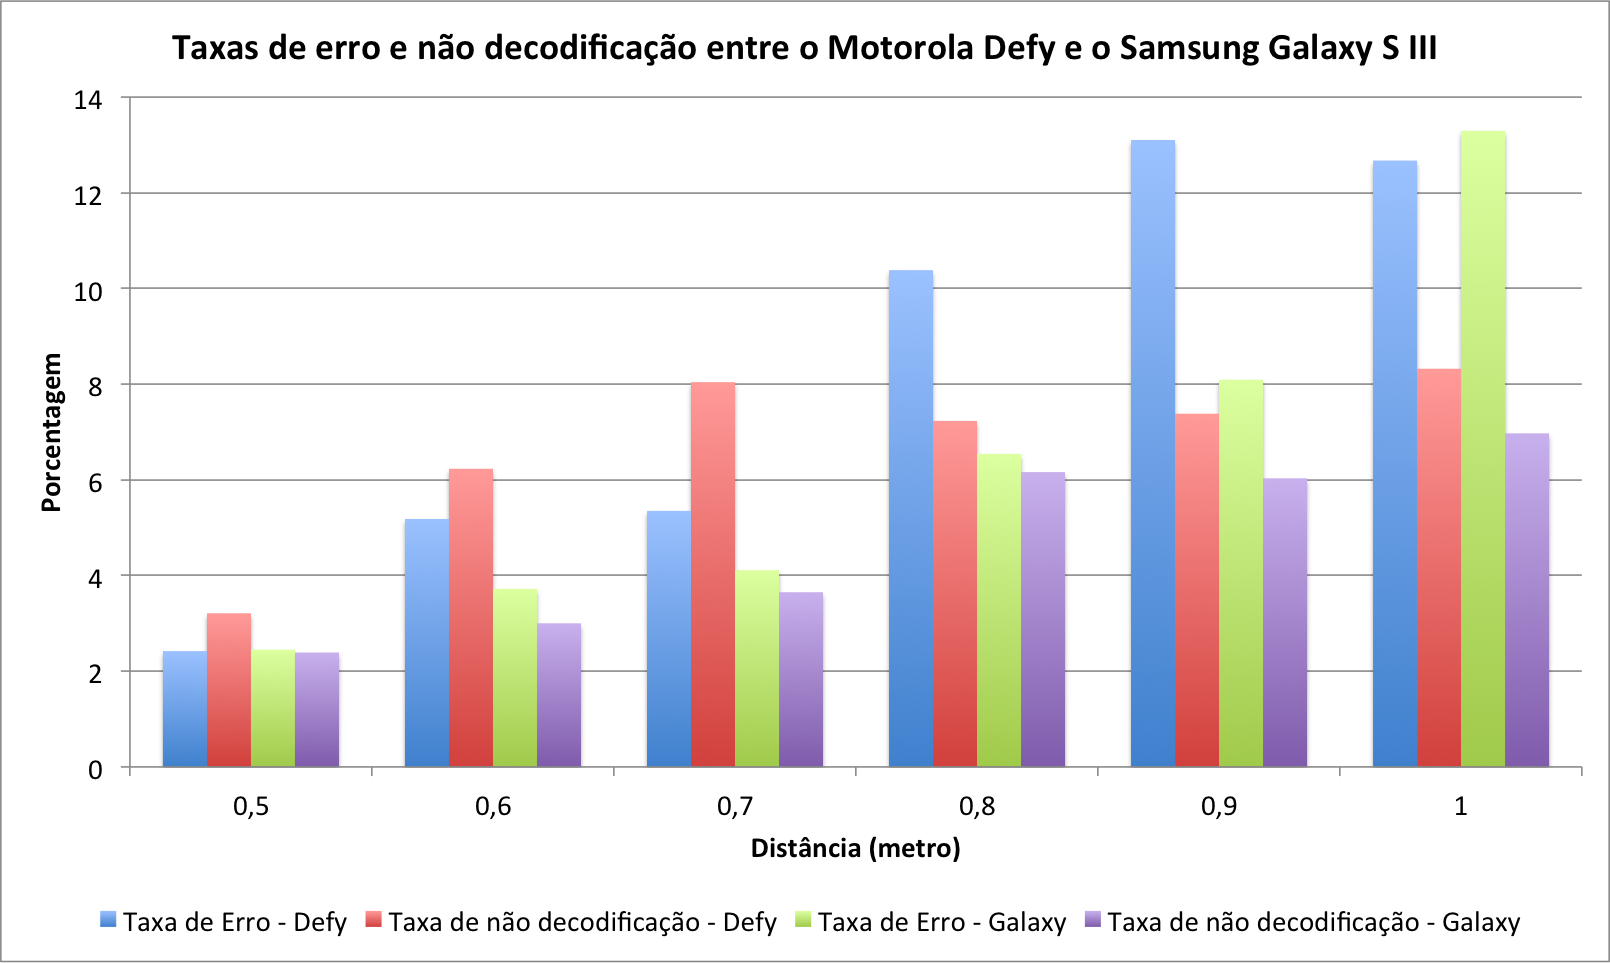
\includegraphics[scale=0.55]{figuras/cap4/grafico_taxas_defy_s3.png}
		\caption{\textit{Comparativo entre as taxas de erro e de não decodificação da aplicação ARHydra entre os 
						dispositivos Motorola Defy e Samsung Galaxy SIII.}}
		\label{fig:testeCompTaxas} 
	\end{figure}
	
	A Figura~\ref{fig:testeCompTaxas} apresenta as Taxa de Erros e Taxa de não decodificação. Novamente o Galaxy SIII 
	mostrou superioridade na maioria das distâncias avaliadas. Esses resultados demonstram a influência da qualidade 
	da imagem capturada em relação as taxas aqui apresentadas. Não levando em consideração as etapas voltadas ao 
	pré-processamento de imagens que possam ser implementadas na ARHydra, conclui-se então que quanto maior for a qualidade da 
	câmera (resolução, qualidade das lentes, algoritmo utilizado na compressão das imagens, controle de luminosidade, etc), 
	juntamente com a melhoria na qualidade dos valores recebidos pelo sensor de orientação do~\textit{smartphone}, menores 
	serão as taxas de erro e decodificação apresentadas na ARHydra. 
	
\subsubsection{Suporte a diversas aplicações de decodificação do QRCode}

	A ARHydra permite a integração de diferentes mecanismos para a decodificação de QRCodes a serem utilizados no Módulo 
	de decodificação. Na atual versão da aplicação é permitido utilizar tanto a implementação fornecida pelo ZBar e o 
	ZXing para esta tarefa. Tomando esta flexibilidade como base, foram realizados testes para verificar o comportamento 
	fornecido por cada um destes. 
	
	Para estes testes foi utilizado o~\textit{smartphone} de melhor capacidade, o Samsung Galaxy SIII, de forma que o 
	nível de tolerância a falhas do QRCode foi ajustado para o modo~\textit{Quality}. Neste teste 
	foram obtidas quinhentas medições por posição em cada implementação. Os resultados obtidos podem ser observados na 
	Figura~\ref{fig:testeSuporte}.
	
	\begin{figure}[htb] 
		\centering 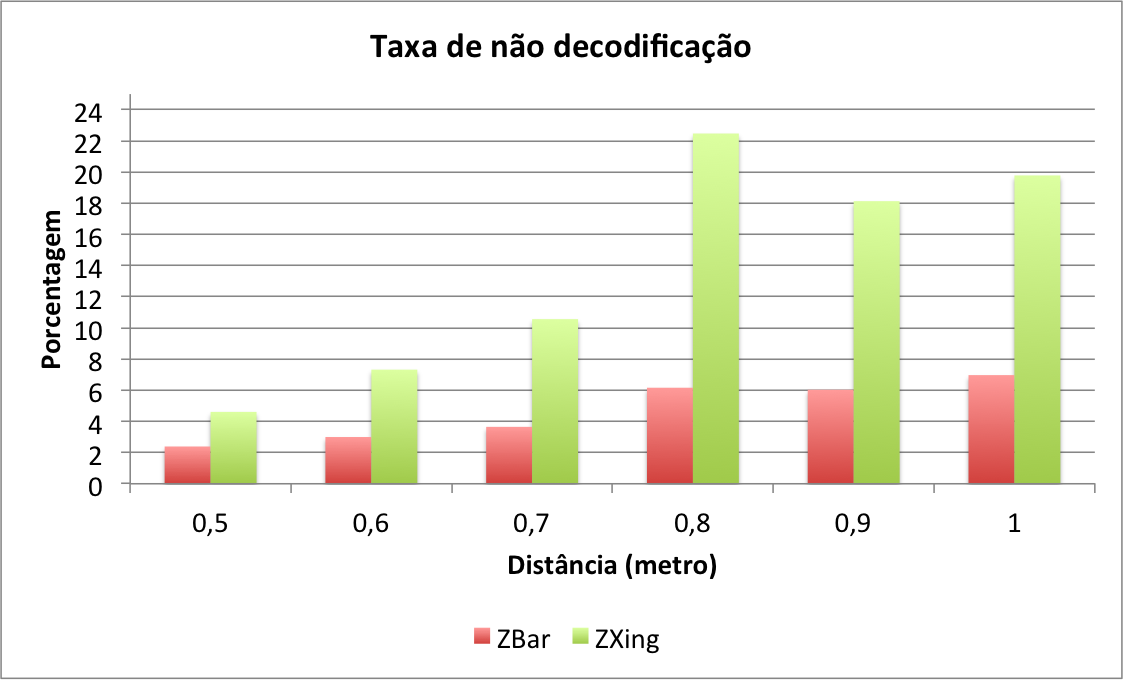
\includegraphics[scale=0.75]{figuras/cap4/grafico_suporte.png}
		\caption{\textit{Taxa de não decodificação para as aplicações ZBar e ZXing.}}
		\label{fig:testeSuporte} 
	\end{figure}
	
	Os resultados apresentados indicam que a implementação ZBar apresenta taxas de não decodificação mais baixas do 
	que a ZXing. Na maioria das distâncias analisadas, ambas as aplicações apresentaram aumento em suas taxas a 
	medida com que a distância fosse aumentada. A diferença apresentada nos resultados está relacionado ao algoritmo 
	utilizado por essas aplicações, porém não foi possível obter informações a respeito da implementação dos mesmos.
	
	
\subsubsection{Influência da tolerância a falhas do QRCode}

	%Estes níveis tem por objetivo facilitar a decodificação do QRCode, porém o formato do 
	%local de armazenamento de seu conteúdo varia de acordo com seu nível de tolerância a falhas implementado.
	
	Como visto na seção \ref{sec:simbolos_bidimensionais}, os QRCodes podem ser compostos por quatro níveis de 
	tolerância a falhas. Este conjunto de testes por sua vez, visa estabelecer um parâmetro de qual nível seria 
	melhor aplicado à aplicação ARHydra, uma vez que a longa distâncias a câmera não consegue capturar os pontos 
	do QRCode, impossibilitando	assim sua decodificação. 
	
	Para análise dos resultados foram realizadas quinhentas medições para cada distância, sendo esta 
	repetida para todos os níveis de tolerância a falhas. Por fim, o módulo de decodificação foi configurado 
	para utilizar a	aplicação ZBar nos testes mencionados, devido suas melhores taxas obtidas no teste anterior. 
	
	\begin{figure}[htb]
		\centering 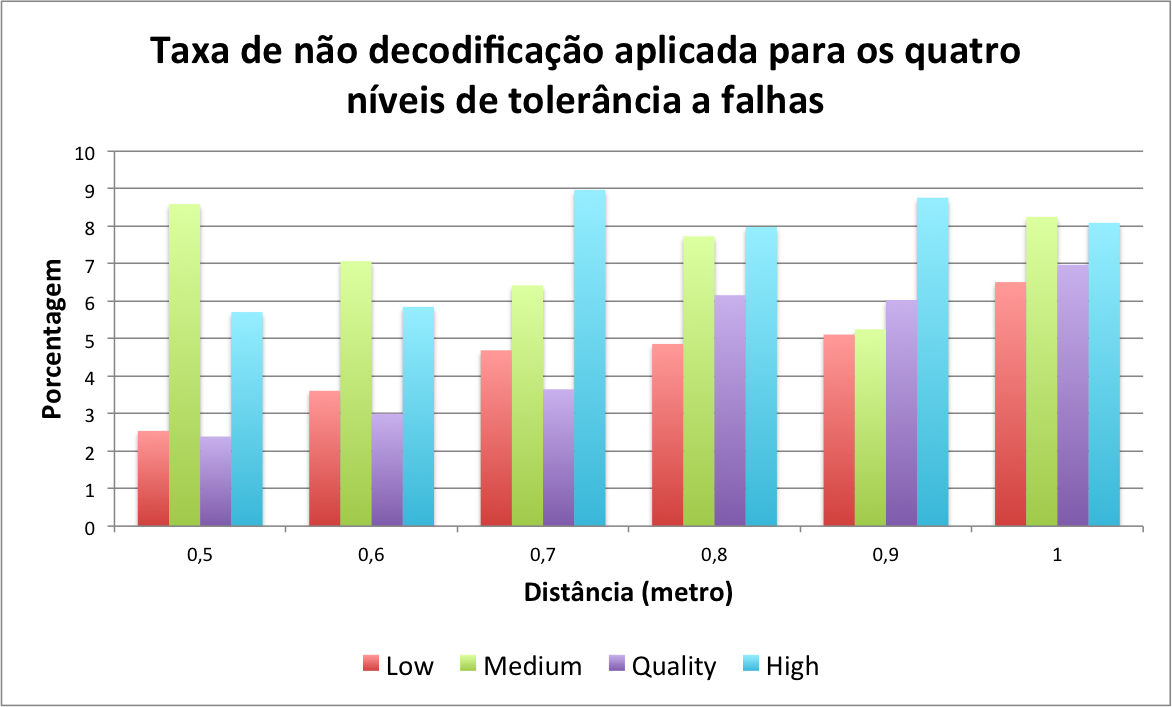
\includegraphics[scale=0.75]{figuras/cap4/grafico_nivel_decode.png}
		\caption{\textit{Nível da taxa de não decodificação aplicado sobre a influ{\^e}ncia da toler{\^a}ncia a falhas do QRCode.}}
		\label{fig:testeNivelDecode} 
	\end{figure}
	
	A Figura \ref{fig:testeNivelDecode} apresenta os resultados para este teste. Estes níveis possuem percentuais de 
	recuperação a falhas conforme a Tabela~\ref{tab:nivelFalha}. Os marcadores, quando ajustados aos 
	níveis~\textit{Low} e~\textit{Quality}, obtiveram melhores resultados comparado aos demais níveis. Embora, as taxas 
	de todos os níveis tenham apresentado aumento à medida que o dispositivo se afastava do marcador em questão. Quando 
	os níveis~\textit{Low} e~\textit{Medium} são comparados, é possível observar que o formato de seus campos responsáveis
	pela estruturação do QRCode, mesmo quando a diferença na porcentagem da tolerância a falhas é pequena, interfere na 
	obtenção dos pontos	internos ao código, ocasionando uma variação muito grande na taxa de não decodificação. 
	Esse mesmo comportamento é observado para os níveis~\textit{Quality} e~\textit{High}. 
	
	A medida com que é elevado o nível de tolerância a falhas há um aumento da quantidade de informação a ser armazenada
	para cobrir a porcentagem de informação que pode ser recuperada. No entanto, o espaço ocupado pelo QRCode, no marcador 
	utilizado, permaneceu o mesmo, independente do nível de recuperação a falhas aplicado. Desta forma, quanto maior o nível de 
	recuperação a falhas utilizado mais complexo será a decodificação do marcador utilizado. A partir dos resultados 
	analisados, conclui-se que o nível~\textit{Low} de tolerância a falhas é o que melhor se aplica para utilização na 
	aplicação ARHydra para as distâncias analisadas. 
	
	
	
		 
	


	\chapter{Conclusão}
\label{cap:conclusao}
%\epigraph{`` Colocar algo. ”}{Autor}
	 
	
	Com a evolução da computação móvel, os~\textit{smartphones} tornaram-se mais presentes em nosso dia a dia devido as
	crescentes funcionalidades que oferecem aos usuários. Estes, por sua vez, podem ser 
	compartilhados dentro da~\textit{ubicomp}, através do acesso aos seus serviços pelos demais
	dispositivos inseridos dentro do~\textit{smart space}. É neste cenário que se insere a construção de mecanismos que 
	simplifiquem a integração e visualização dos recursos. Seu intuito é que o usuário descubra de forma mais simples as 
	opções que se encontram no ambiente a sua volta.
	 
 	A aplicação ARHydra (\textit{Augmented Reality Hydra}) surgiu a partir dessa dificuldade em se localizar
 	e utilizar os recursos dos dispositivos no~\textit{smart space}. Tomando por base os conceitos de adaptabilidade de 
 	serviços providos pela DSOA, aplicado ao~\textit{middleware uOS}. A aplicação auxilia o usuário a localizar, 
 	visualizar e redirecionar os recursos presentes no ambiente inteligente através do uso de 
 	recursos da Realidade Aumentada e pela sua integração com a aplicação Hydra. 
 	
 	 	
 	Foram conduzidos conjuntos de testes cujo objetivo fosse validar a proposta desse trabalho. Como foi possível 
 	verificar com os testes apresentados na seção~\ref{sec:resultados}, a aplicação ARHydra operou de forma bastante
 	satisfatória para os resultados apresentados para estes testes.	Os resultados apresentaram a influência da 
 	qualidade na captura das imagens pelas câmeras. Essa qualidade não é caracterizada somente pela 
 	resolução da câmera, mas também por uma série de fatores que possam divergir no resultado mesmo quando aplicados 
 	nas mesmas condições de uso. Por essa razão, faz-se necessário aplicação de etapas de pré-processamento de 
 	imagens para minimizar este problema.
 	
 	Adicionalmente, os testes realizados voltados para validação da troca de informação, pelo do Módulo de Integração, 
 	entre as aplicações ARHydra e Hydra foram desenvolvidos utilizando o~\textit{framework} Junit. 
 	Através destes, comprovou-se a correta implementação dos objetivos propostos por este trabalho, facilitando ao 
 	usuário encontrar, visualizar e redirecionar um determinado	recurso à Hydra em poucos segundos, demonstrando ser 
 	uma boa forma de interação com a Hydra. No entanto, os testes demonstraram 
 	uma fragilidade da implementação da Hydra para o redirecionamento dos recursos de câmera e tela, implementados 
 	utilizando o JMF (\textit{Java Media Framework}), fazendo com que algumas vezes o redirecionamento não ocorra de
 	conforme o esperado.
 	
 \section{Trabalhos Futuros}

	A aplicação ARHydra tornou possível a interação dos usuários com o~\textit{smart space} de forma 
	mais intuitiva, combinando os recursos providos pela Realidade Aumentada e os princípios envolvidos
	pela~\textit{ubicomp}. Essa interação acrescentou mais características ubíquas a Hydra e proporcionou facilidades 
	ao usuário na visualização e seleção dos recursos inseridos dentro do ambiente inteligente, possibilitada 
	através da integração entre dessas duas aplicações. 
	
	Com o desenvolvimento da ARHydra, abre-se caminho para melhorias e novos desenvolvimentos. Dentre as melhorias 
	podemos citar: 
	
	\begin{enumerate}
	  
	  \item Ampliação no reconhecimento dos marcadores para que a aplicação consiga identificar e interagir com 
	  		múltiplos marcadores ao mesmo tempo, expandindo as possibilidades observados pelo usuário.
	  
	  \item Localização e reconhecimento de marcadores dentro de imagens mais complexas, possibilitando a implementação 
	  		de técnicas de pré-processamento de imagens para aumentar a qualidade do reconhecimento e decodificação do 
	  		QRCode, podendo minimizar os problemas decorrentes da captura dessas imagens em ambientes com pouca luminosidade. 
	   
	  \item Implementação de um mecanismos que identifique e armazene os marcadores que	foram reconhecidos. Atualmente, 
	  		a não implementação deste mecanismo faz com que cada reconhecimento seja reprocessado a partir do início.
			
	  \item Devido a mobilidade dos dispositivos inseridos no~\textit{smart space} poderia 
			ser desenvolvido uma integração	da ARHydra com tecnologias baseadas em rádio frequência, conforme visto 
			na seção~\ref{sec:smart}, de forma com que o~\textit{uOS} ficasse responsável pelo gerenciamento e 
			atualização do posicionamento dos objetos. Deste modo, o~\textit{uOS} disponibilizaria essas informações
			através de um um canal de comunicação com a ARHydra onde essas informações poderiam ser atualizadas a cada
			novo reconhecimento.     
			
	  \item Adaptação da aplicação ARHydra para sua utilização com outros tipos marcadores, que não utilizem o 
	  		QRCode para armazenamento de informações a respeito do dispositivo.
	  		
	\end{enumerate}


	%\anexos
	%

\chapter{Android}
	
	%TODO verificar o que esse middleware faz
	Android é um projeto ~\textit{open source} iniciado pela Google, voltado para plataformas de
	dispositivos móveis desenvolvido na linguagem Java, incluindo sistema operacional,
	~\textit{middleware} e aplicações chaves. Inicialmente os celulares não possuíam muita memória,
	isso fazia com que as aplicações Java consumissem boa parte dessa memória. Para contornar esse
	problema, foi desenvolvido uma nova ~\textit{Virtual Machine (VM)} específica denominado de
	~\textit{Dalvik Virtual Machine (DVM)} ~\cite{android}.
	
	Colocar um comentário melhor:
	
	\begin{itemize}
	  \item {~\textit{Dalvik Virtual Machine \\}}
	  
			O ~\textit{DVM} possui um comportamento um pouco diferente quando comparado a ~\textit{JVM}.
			Enquanto que na ~\textit{JVM} a compilação de classes classe gera um arquivo .class específico
			para cada classe, no ~\textit{DVM} a compilação das classes gera um arquivo de extensão
			~\textit{dex} contendo várias classes. O arquivo gerado é otimizado para o melhor uso da memória e
			operações de entrada e saída. \\
	  
	  \item  {~\textit{Software Development Kit} \\}
		
		O Android possui um ~\textit{Software Development Kit (SDK)} próprio. Neste ~\textit{SDK} são
		disponibilizados os recursos necessários para o desenvolvimento das aplicações no ambiente Android
		e trás a possibilidade de emulação de diversos dispositivos para testes dessas aplicações. \\
		
	  \item {~\textit{Native Development Kit} \\}		
	
		A plataforma do Android aceita aplicações que sejam desenvolvidas com a linguagem Java. No entanto,
		é possível combinar aplicações Java com aplicações e bibliotecas desenvolvidas em C/C++ utilizando
		a ~\textit{Java Native Interface (JNI)} através do ~\textit{Native Development Kit (NDK)}. \\
	
	\end{itemize}

	\section{Arquitetura}
	
		A figura ~\ref{androidArquitetura} apresenta como a arquitetura do Android está dividida em camadas.
		Sendo estas divididas em:
	
		\begin{itemize}
			\item{ ~\emph{Aplications} \\}
			
				Nesta camada ficam as aplicações propriamente ditas, as quais são manipuladas pelo usuário
				final. Sendo composta por funções básicas do dispositivo, como por exemplo, realizar chamada,
				navegar na internet, acessar lista de contatos, dentre outras. \\
			
			\item{~\emph{Aplication Framework} \\}
			
				Descendo para a próxima camada temos a camada responsável pelas funções de gerenciamento do
				telefone. Nesta camada é possível encontrar um conjunto de componentes voltados para o auxílio
				no desenvolvimento de aplicações, disponibilizadas em ~\textit{Application Programming Interface
				(API)} e recursos necessários para os pacotes e aplicativos, tais como classes visuais (botões
				e ~\textit{views}), troca de recursos entre aplicativos, gerenciamento dos recursos, ciclo de
				vida de aplicações e gerenciamento de pacotes. \\
					
			\item{~\emph{Libraries} \\}
			
				Aqui são incluídas as bibliotecas do Android, muitas delas desenvolvidas em C/C++ e são
				utilizadas por diversos componentes do sistema. Estas bibliotecas possuem conjuntos de
				instruções que facilitam o desenvolvimento de aplicações, dando suporte a camada superior.
				O conjunto de bibliotecas extende-se desde a manipulação de arquivos de mídia, imagem e vídeo,
				oferecendo suporte a exibição de conteúdos bidimensionais e tri diomensionais, baseados no
				OpenGL, chegando até a manipulação de dados em banco de dados com o SQLite.\\
				
			\item{~\emph{Android Runtime} \\}
			
				É nesta camada que o ~\textit{DVM} reside e divide espaço com as bibliotecas principais do
				sistema. Essas bibliotecas fornecem a maioria das funcionalidades disponíveis. Um ponto interessante
				implementado nessa arquitetura é a utilização de instâncias ~\textit{DVM} para cada processo, ou
				seja, cada aplicação possui seu próprio processo e sua própria instância da ~\textit{DVM}. \\

			\item{~\emph{Linux Kernel} \\}
			
				Essa camada atua como uma camada de abstração entre o hardware e o software. Fica responsável
				pelo gerenciamento de memória e processos, rede e ~\textit{drivers} de conexão. \\
				
		\end{itemize}
	
	
		\begin{figure}[h]
			\centering 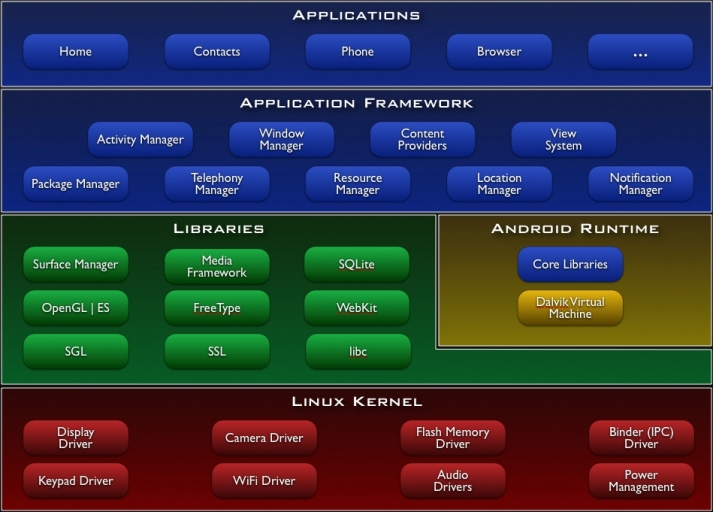
\includegraphics[scale=.65]{figuras/anexos/androidArquitetura.jpg}
			\caption{\textit{Arquitetura do Android ~\cite{android}.}}
			\label{androidArquitetura} 
		\end{figure}
	



	
	\postextual
	
	\bibliographystyle{plain}
	\bibliography{bibliografia}

\end{document}
